\documentclass{article}
\usepackage{graphicx} % Required for inserting images
\usepackage[T1]{fontenc}
\usepackage[utf8]{inputenc}
\usepackage[catalan]{babel}
\usepackage{hyperref}
\usepackage{url}
\usepackage{float}
\usepackage{tabularx}
\usepackage{amsmath}
\usepackage{xcolor,colortbl}
\usepackage{caption}
\usepackage{subcaption}
\usepackage{algorithm}
\usepackage{algpseudocode}
\usepackage{amsmath}
\usepackage{pdfpages}

\definecolor{Gray}{gray}{0.85}

\title{\bfseries Simulation and visualization of lichens growth in cultural heritage 3D models \normalfont \vspace{0.3cm} \\ \large Quarta entrega GEP \\ \vspace{1cm} Treball de Fi de Grau \\ \vspace{0.3cm} Grau en Enginyeria Informàtica FIB-UPC \vspace{10cm}}
\author{Autor: Roc Salvador Andreazini \\ Directors: Imanol Muñoz i Oscar Argudo}
\date{\today}

\begin{document}

\includepdf[pages=-]{portada.pdf}

\newpage

\textbf{\large Resum}

\paragraph{} Els models d'herència cultural són representacions virtuals de monuments històrics. La seva funció és preservar i permetre visites a distància d'aquests monuments, aquest projecte se centra en el model virtual de l'església de Pedret. Proposo un mètode per simular el creixement i la visualització de líquens per al model de Pedret per tal de millorar-ne el realisme i fer-lo més fidel i més atractiu als visitants. Aquest mètode permet generar textures de líquens realistes des de zero, és a dir, que a partir d'uns paràmetres se simuli el creixement dels líquens i després es creï una visualització fidedigna que es pugui aplicar al model directament.

\paragraph{} Paraules clau: Líquens, textures, dla, models d'herència cultural.

\newpage

\textbf{\large Abstract}

\paragraph{} Cultural heritage models are virtual representations of historical monuments. Their function is to preserve and enable remote visits to these monuments. This project focuses on the virtual model of the Church of Pedret. I propose a method to simulate the growth and visualization of lichens for the Pedret model to enhance its realism, make it more faithful and attractive to visitors. This method allows the generation of realistic lichen textures from scratch, meaning that lichen growth is simulated from certain parameters, and then a faithful visualization is created that can be directly applied to the model.

\paragraph{} Keywords: Lichens, textures, dla, cultural heritage models.

\newpage

\tableofcontents

\listoffigures

\listoftables

\newpage

\section{Context}

Aquest TFG és dirigit pels doctors Imanol Muñoz i Oscar Argudo dins de l'especialitat de Computació de la FIB.

\subsection{Introducció}

Aquest TFG s'emmarca en el projecte EHEM (Enhancement of Heritage Experiences: the Middle Ages. Digital Layered Models of Architecture and Mural Paintings over Time) \cite{EHEM}. Projecte en el qual els dos directors del TFG estan involucrats a través del grup de recerca VIRVIG \cite{virvig}. L'objectiu d'aquest projecte és preservar i mostrar totes i cadascuna de les capes d'un seguit d'esglésies medievals amb pintures murals mitjançant models 3D realistes que permeten conservar-les, actualitzant els models periòdicament incorporant els resultats de noves investigacions i difonent-los. 

Un exemple dels tres models d'herència cultural (\textit{cultural heritage models} en anglès) en els quals treballa l'EHEM i en el que ens centrarà aquest treball és l'església preromànica de Sant Quirze de Pedret (Cercs, Berguedà) datada del segle X.

\begin{figure}[H]
    \centering
    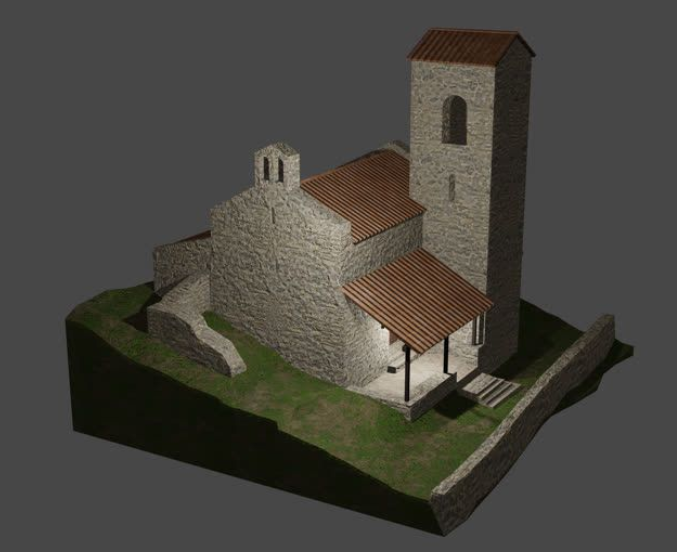
\includegraphics[width=0.5\linewidth]{img/misc/church.png}
    \caption{Model 3D de l'església de Sant Quirze de Pedret. Imatge extreta de la pàgina web de l'EHEM \cite{EHEM}}
    \label{fig:enter-label}
\end{figure}

La meva tasca dins d'aquest projecte és la de dotar de més realisme als models afegint líquens que creixen i s'adapten a les condicions on se situa el model.

\begin{figure}[H]
    \centering
    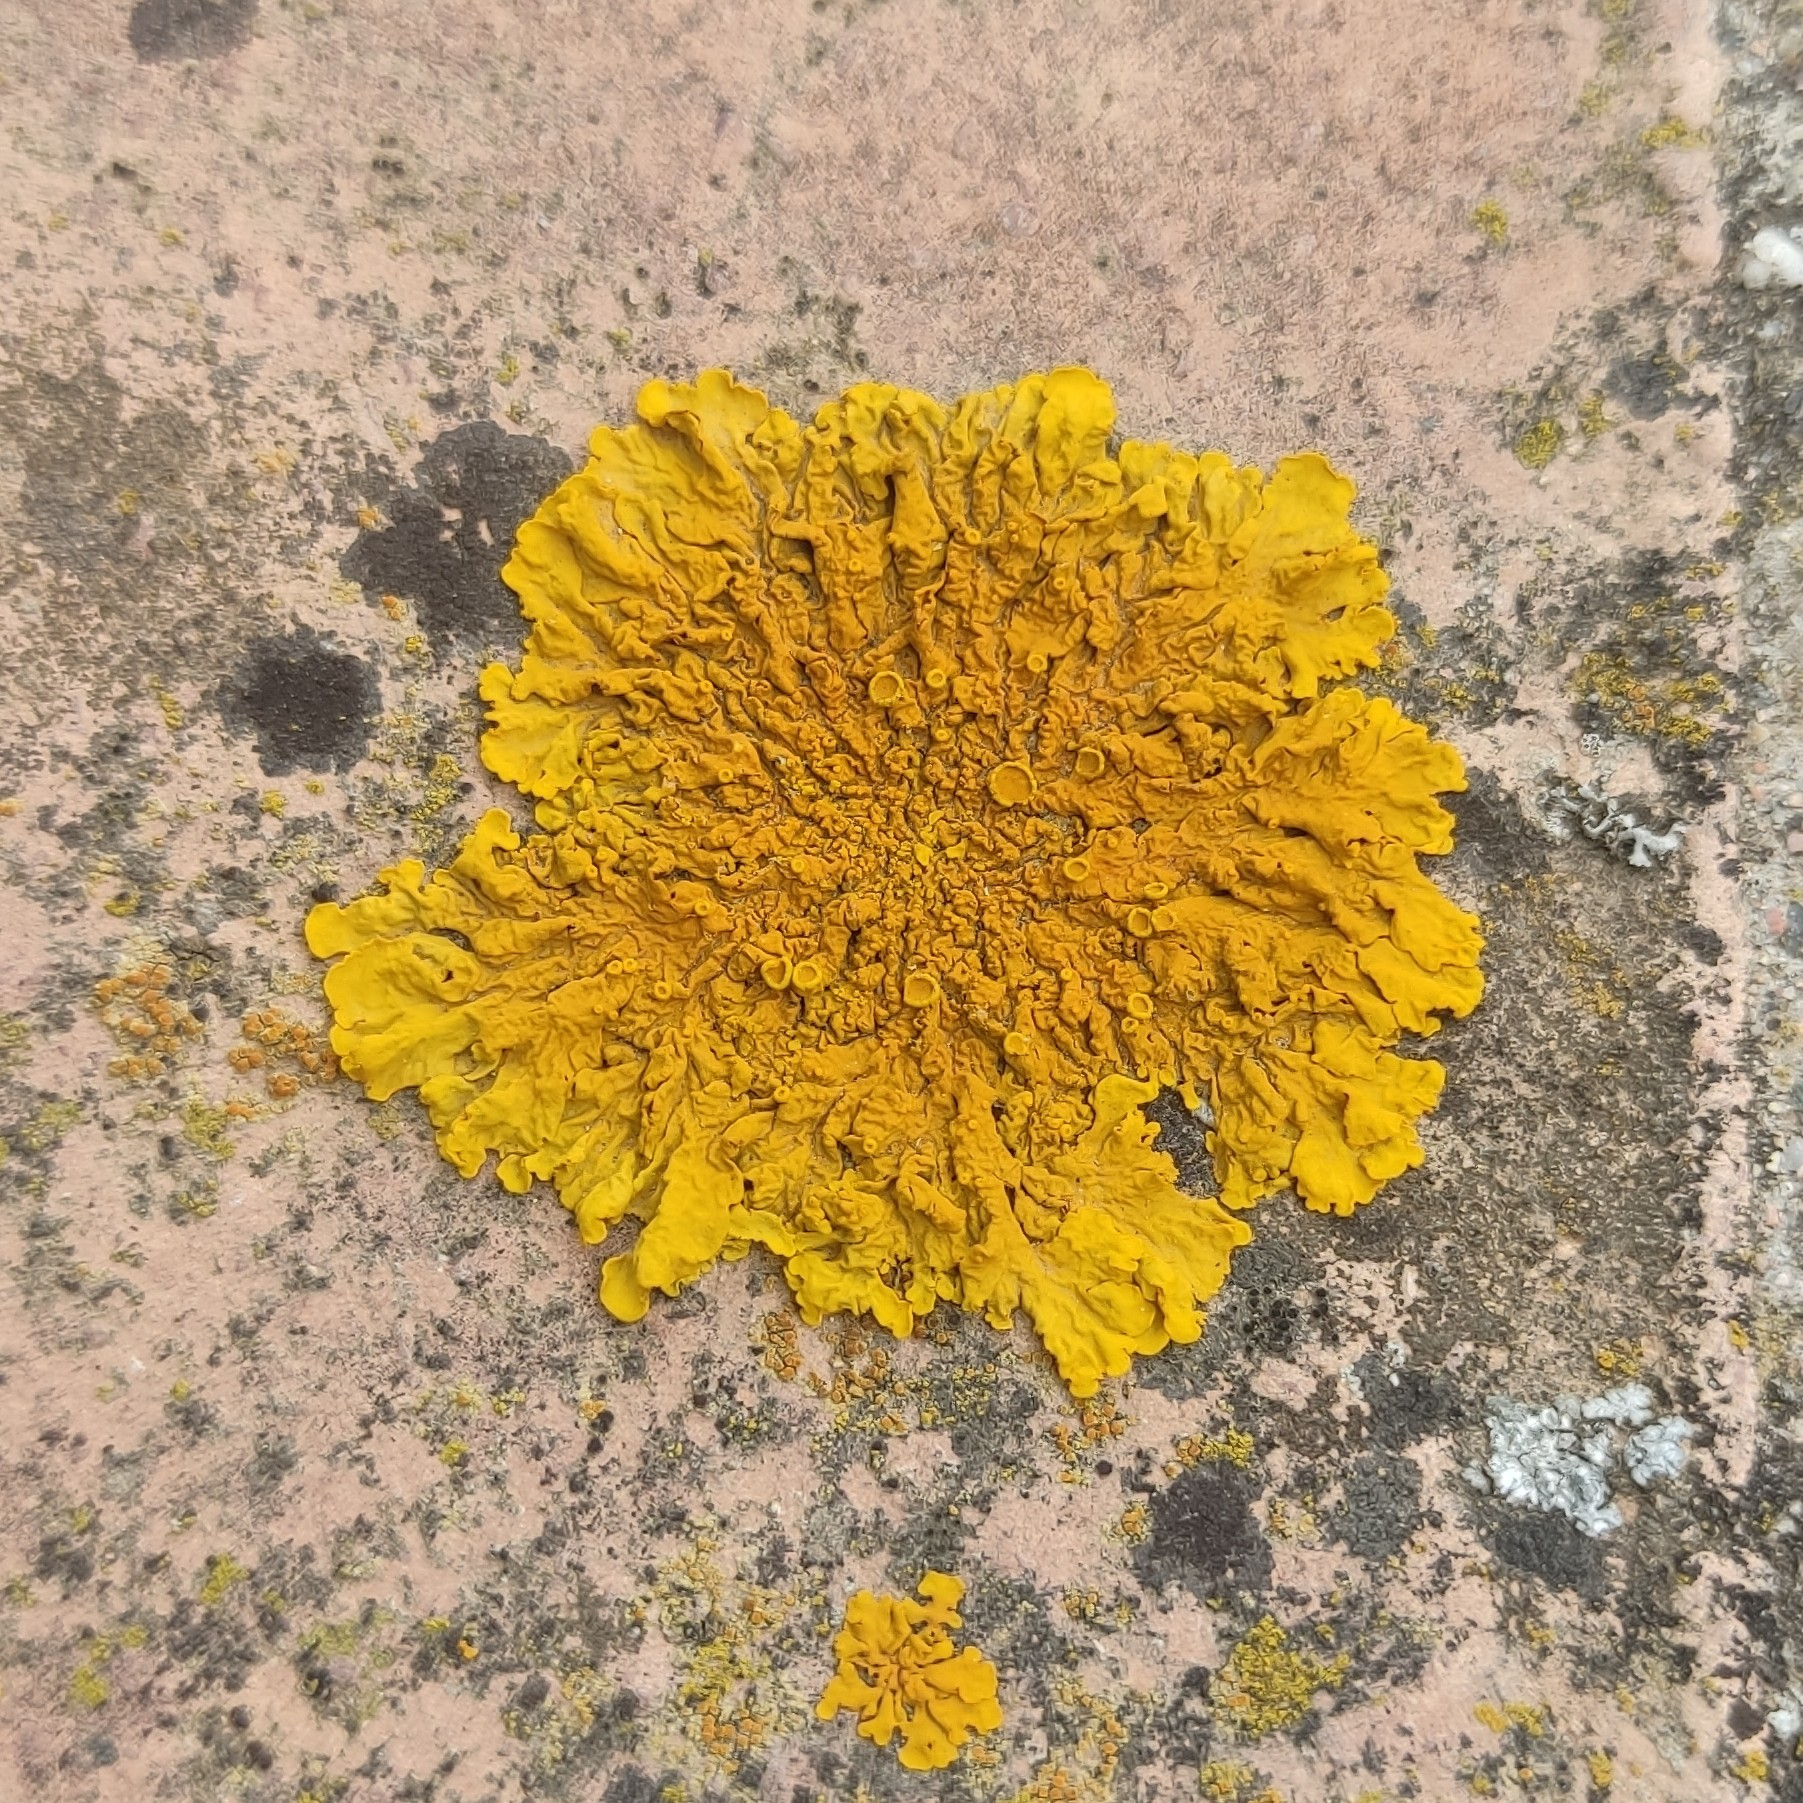
\includegraphics[width=0.5\linewidth]{img/misc/liquen.jpg}
    \caption{Fotografia d'un liquen. Font: Oscar Argudo.}
    \label{fig:real-lichen}
\end{figure}
\subsection{Conceptes}

Per tal que el treball sigui més entenedor, primer s'han de definir els conceptes recurrents i específics d'aquest treball.

\begin{itemize}
    \item Textura: Una textura és un mapa de bits que s'utilitza per cobrir un objecte virtual. Cada punt de la textura, anomenat texel, correspon a les dades d'un punt de la superfície del model. N'existeixen diferents tipus que tenen diferents funcions per a la visualització final dels objectes. 
    \begin{itemize}
        \item Mapa de normals: El mapa de normals conté el valor de la normal per cada punt de la textura codificat en RGB. Aquests valors es poden utilitzar després per obtenir una il·luminació més realista.
    \begin{figure}[H]
        \centering
        
\includegraphics[width=0.6\textwidth]{img/misc/normal_mapping.png}
        \caption{Escena tridimensional (esquerra). Exemple d'un \textit{normal mapping} (centre), calculat a partir de l'escena tridimensional. Resultat quan s'aplica a una superfície plana (dreta). Font: Wikimedia Commons \cite{wikimediaWikimediaCommons}.}
        \label{fig:enter-label}
    \end{figure}
        \item Mapa de colors: El mapa de colors conté la informació del color per cada punt de la textura. Aquesta informació es fa servir per afegir color a l'objecte on s'aplica la textura.
        \item Mapa de rugositat: El mapa de rugositat indica la llisor de cada punt de la textura. Aquests valors s'utilitzen per indicar com interactua la llum amb l'objecte, reflectint més o menys d'aquesta.
    \begin{figure}[H]
        \centering
        
\includegraphics[width=0.6\textwidth]{img/misc/roughness_map.png}
        \caption{Exemple de l'efecte de la rugositat (\textit{roughness} en anglès) en un mateix objecte. Font: Wikimedia Commons \cite{wikimediaWikimediaCommons}.}
        \label{fig:enter-label}
    \end{figure}
        \item Mapa de desplaçament: El mapa de desplaçament conté la informació de l'alçada de cada punt de la textura. Aquesta informació serveix per afegir relleu a l'objecte on s'aplica.
        \begin{figure}[H]
            \centering
            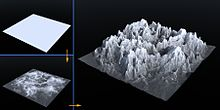
\includegraphics[width=0.6\textwidth]{img/misc/displacement_map.jpg}
            \caption{Exemple de mapa de desplaçament (avall a l'esquerra) aplicat a un pla (dreta). Font: Wikimedia Commons \cite{wikimediaWikimediaCommons}.}
            \label{fig:enter-label}
        \end{figure}
    \end{itemize}
    \item DLA (Diffusion Limited Aggregation): El DLA és un algorisme que consisteix a crear partícules en posicions aleatòries i moure-les aleatòriament, mitjançant el que s'anomena en anglès \textit{random walks}. Aquestes partícules es mouen fins que s'agreguen a una altra partícula. La forma que genera un DLA depèn de la manera com es calcula la probabilitat que una partícula s'agregui amb una altra.
    \begin{figure}[H]
        \centering
        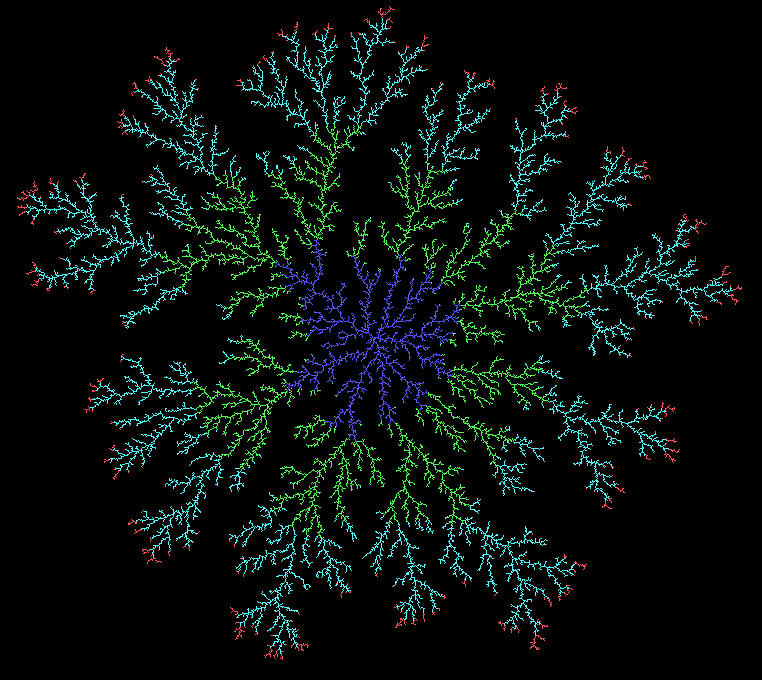
\includegraphics[width=0.6\textwidth]{img/misc/dla.jpg}
        \caption{Exemple d'un DLA generat mitjançant \textit{random walks}. Font: Wikimedia Commons \cite{wikimediaWikimediaCommons}.}
        \label{fig:enter-label}
    \end{figure}
\end{itemize}

\subsection{Definició del problema}

Un dels factors més importants dels models virtuals de monuments culturals és la fidelitat amb la qual representen la realitat, per preservar correctament els monuments i fer més atractiu al públic general visites a través d'aquests models virtuals. El que pretén aquest TFG és afegir una capa més de realisme als models d'herència cultural amb la presència de líquens que s'adapten a les condicions als materials on apareixen i a les condicions meteorològiques de l'entorn on es localitza el model.

\subsection{Actors implicats}

Els actors implicats en qualsevol projecte es divideixen entre actors interns i els actors externs. 

Els actors interns són els que influeixen directament en el projecte. En el cas d'aquest TFG serien:

\begin{itemize}
    \item Autor (Roc Salvador): Investiga, desenvolupa i escriu l'informe final. 
    \item Directors (Imanol Muñoz i Oscar Argudo): Avaluen i guien l'evolució del projecte per tal que segueixi els objectius que tenien al cap en proposar el projecte. 
\end{itemize}

Els actors externs són els que es veuen beneficiats o afectats pels resultats d'aquest TFG. En el cas d'aquest treball són:

\begin{itemize}
    \item Investigadors del grup de recerca ViRVIG: Directament beneficiats, ja que és part de la seva feina dins del projecte EHEM.
    \item Participants en el projecte EHEM: Els resultats ajudaran a millorar els models que es desenvolupen en aquests, ja que un dels objectius d'aquest treball és que serveixi per a qualsevol model.
    \item Investigadors en el camp dels gràfics i l'algorísmia: les modificacions d'eficiència que es fan del model poden ser interessants des del punt de vista de complexitat computacional i, per altra part, el procés que desenvolupem per generar les textures pot ser interessant des del punt de vista de la computació de gràfics.
    \item Públic general: Se'n veu beneficiat gràcies al fet que els resultats d'aquest treball donen més realisme als models que poden visitar de manera virtual.
\end{itemize}

\newpage

\section{Justificació}

\subsection{Estudis previs}

Existeixen diferents algorismes per a la generació de patrons que simulen la forma dels líquens a la vida real, molts d'aquests articles estan dedicats exclusivament a la generació dels patrons. És per això que d'entre tots els articles que toquen aquest tema he decidit basar la simulació i visualització dels líquens en l'article \textit{Simulating and modeling lichen growth} \cite{Simulating-and-modeling-lichen-growth}, ja que parla específicament de com modelar les diferents condicions, ja siguin climàtiques (llum del sol o temperatura) o condicions dels materials on creix els líquens.

\subsection{Justificació}

El que ens permet agafar un algorisme existent és centrar-nos a millorar-lo per a les nostres necessitats donats els coneixements i els temps limitats que tinc per a fer el treball. A més, com que el treball es divideix en dues seccions (generació del liquen i generació de les textures), ens permet centrar-nos més temps a millorar com es veuran els líquens en el model, factor molt important, ja que un dels principals objectius del treball és de dotar de realisme als models d'herència cultural.

\newpage

\section{Abast}

\subsection{Objectius i subobjectius}

El projecte es divideix en dos objectius principals molt diferenciats entre ells i aquests en subobjectius més concrets:

\begin{itemize}
    \item Desenvolupar un algorisme basat en el de l'article \textit{Simulating and modeling lichen growth}  \cite{Simulating-and-modeling-lichen-growth} que satisfaci les característiques necessàries per al model d'herència cultural.
    \begin{itemize}
        \item Desenvolupar una versió eficient de l'algorisme original i millorar l'eficiència per al cas concret en què el farem servir.
        \item Afegir paràmetres que ens semblin necessàries a l'algorisme original.
    \end{itemize}
    \item Desenvolupar una pipeline que a partir de la sortida del DLA generi els mapes de textura per al model.
    \begin{itemize}
        \item Generar les imatges de les textures a partir dels resultats del DLA.
        \item Mitjançant Blender, afegir al model les textures generades anteriorment.
    \end{itemize}
\end{itemize}

\subsection{Requeriments}

\begin{itemize}
    \item Funcionals
    \begin{itemize}
        \item Simular el creixement dels líquens segons les condicions climàtiques i del material on creixen.
        \item Generar les textures correctament sobre el material donat.
    \end{itemize}
    \item No funcionals
    \begin{itemize}
        \item Eficiència: l'algorisme DLA ha de ser eficient, ja que és possible que es generin molts líquens.
        \item Configurabilitat: s'han de poder modificar el màxim de paràmetres possibles que defineixen el creixement d'un liquen.
        \item Modularitat: Tant l'algorisme DLA, com la generació de textures han de funcionar independentment. És a dir, si es vol generar només l'estructura del DLA o només les textures a partir d'una estructura donada, s'ha de poder.
        \item Reusabilitat: La generació de líquens hauria de funcionar per qualsevol model.
    \end{itemize}
\end{itemize}

\subsection{Obstacles i riscos}

Com a qualsevol projecte de recerca, no se sap quins resultats s'obtindran i això planteja diferents riscos. A més, durant la realització del treball se'ns poden presentar diferents obstacles per avançar cap al nostre objectiu.

\begin{itemize}
    \item Termini del projecte: Tenim un temps limitat per fer el projecte, per tant, qualsevol contratemps pot fer que no arribem a temps a complir algun dels objectius.
    \item Inexperiència en recerca: És el primer projecte en el qual faig recerca com a tal en el camp de la informàtica, per tant, és probable que cometi errors.
    \item Problemes informàtics: Qualsevol problema informàtic (pèrdua de fitxers importants, que s'espatlli l'ordinador…) em pot fer perdre temps.
    \item Corba d'aprenentatge de Blender: Blender és un programa molt complex que permet fer coses molt diferents i és la primera vegada que l'uso, per tant, hauré de dedicar temps a aprendre com funciona.
    \item Recursos computacionals limitats: Blender és un programa amb uns requisits alts pel que fa a CPU i a GPU. Tinc un ordinador mínimament potent, però els renderitzats a Blender poden tardar molt de temps.
\end{itemize}

\newpage

\section{Metodologia i rigor}

És important seguir una bona metodologia d'organització, ja que només tenim quatre mesos per entregar el projecte. La metodologia que faré servir s'anomena Kanban i consisteix a dividir la feina en tasques petites que poden ser de tres tipus diferents:

\begin{itemize}
    \item Per fer: Tasques que s'han definit, però encara s'han de dur a terme. 
    \item En progrés: Tasques que en les que s'està treballant.
    \item Finalitzades: Tasques desenvolupament de les quals s'ha acabat.
\end{itemize}

L'eina que utilitzaré per a mantenir el seguiment d'aquestes tasques és Trello, que permet crear diferents targetes amb TODO lists (llistes amb objectius que es poden marcar com a fets a mesura que es completen).

A part de fer el seguiment de les tasques, cada dues setmanes es fa una reunió amb els tutors per tal de revisar com evolucionen les tasques i per poder presentar els meus dubtes.

\subsection{Eines de validació}

Per tal que els directors puguin realitzar un bon seguiment de l'evolució del treball fet per l'autor, s'han fet servir les eines següents:

\begin{itemize}
    \item Google Meet: Per tal de poder fer les reunions de seguiment amb els directors del treball, utilitzarem Google Meet, ja que és una eina fàcil d'utilitzar i té totes les característiques que necessitem. 
    \item Overleaf: Per tal que els directors puguin fer seguiment del progrés que es fa a la memòria, utilitzarem Overleaf que permet compartir documents de LaTeX amb diverses persones amb canvis a temps real.
    \item Google Calendar: Per poder mantenir el seguiment temporal de les fites que decidim a les reunions i per saber quan són aquestes reunions.
    \item Git/GitHub: Per tal de mantenir un historial de modificacions i per tal que els directors les consultin utilitzaré el programari de control de versió Git amb suport de còpia de seguretat al núvol mitjançant GitHub. A més de poder dividir el desenvolupament de codi en diferents branques.
\end{itemize}

\newpage

\section{Descripció de tasques}

El projecte es divideix en dues tasques principals molt clares: la implementació d'un algorisme DLA i la generació de textures realistes a partir dels resultats de l'algorisme. Cada una d'aquestes tasques es divideix en tasques més petites explicades a continuació.

\subsection{Gestió del projecte}

Per tal de fer un millor treball una de les tasques que es fan al principi és la planificació del projecte.

\begin{itemize}
    \item Definició de l’abast i contextualització: Definir el problema, contextualitzar-lo i justificar la tria de la solució que es creu més adequada.
    \item Planificació Temporal: Definir les tasques i organitzar-les en una línia temporal.
    \item Gestió Econòmica i sostenibilitat: Avaluar els costs i la sostenibilitat associats a la realització del projecte.
    \item Document final: Integrar totes les seccions de la gestió del projecte en un document únic.
\end{itemize}

\subsection{Implementació de l'algorisme DLA}

Un dels objectius del treball és implementar un algorisme que generi patrons de líquens basats en el que han proposat per Desbenoit et al. \cite{Simulating-and-modeling-lichen-growth}, per tal de després millorar-lo en eficiència i característiques que es volen pel model en concret. Tenint en compte això, s'han definit les tasques següents:

\begin{itemize}
    \item Llegir l'article i familiaritzar-se amb els conceptes que s'hi presenten.
    \item Implementar l'algorisme tal com es presenta en l'article. 
    \item Afegir les característiques que necessita l'algorisme i millora'n l'eficiència tenint en compte el cas en concret pel qual s'està desenvolupant.
    \item Tests i canvis per millorar la visualització: Provar l'algorisme amb la visualització (l'altra tasca principal) i fer les millores pertinents.
\end{itemize}

\subsection{Generació de textures realistes de líquens}

L'altre objectiu principal és generar les textures dels líquens a partir dels resultats de l'algorisme, integrar el procediment amb Blender i el model d'herència cultural. Les seves tasques seran doncs:

\begin{itemize}
    \item Familiaritzar-se amb els conceptes relacionats amb les textures, per exemple la teoria de com es construeixen aquests mapes i quins tipus n'existeixen.
    \item Aprendre a utilitzar Blender, ja que és una eina molt complexa i complicada d'usar per a un usuari sense experiència.
    \item Crear una \textit{pipeline} per generar les textures a partir de l'algorisme.
    \item Integrar la \textit{pipeline} amb Blender.
    \item Aplicar les textures al model de manera que els líquens creixin en llocs amb sentit i de manera correcta.
\end{itemize}

\subsection{Documentació i defensa del treball}

Les tasques principals no específiques són la redacció del document de la tesi i la defensa del treball davant d'un tribunal.

\begin{itemize}
    \item Documentació: Consisteix a documentar la feina que es va fent de la resta de tasques i redactar el document final.
    \item Preparar la presentació i defensar el treball davant d'un tribunal.
\end{itemize}

\subsection{Recursos}

És important saber de quins recursos es disposa per fer el treball, tant humans com materials.

\subsubsection{Recursos humans}

Els recursos humans són totes les persones involucrades en la realització d'aquest projecte. En aquest cas són: l'autor (Roc Salvador), que recerca, desenvolupa i documenta la solució, els directors, encarregats de la supervisió i guia del projecte i el tutor de GEP que també supervisa i guia, en aquest cas només la Gestió de Projectes.

\subsubsection{Recursos materials}

\begin{itemize}
    \item Overleaf: Editor de LaTeX en línia que permet compartir els documents amb altres usuaris, en aquest cas els directors.
    \item Google Meet: Eina per fer les reunions de seguiment amb els directors.
    \item Google Drive: Eina per compartir fitxers relacionats amb el desenvolupament del projecte amb els directors.
    \item GitHub: Programari de versió de control per mantenir un historial de modificació en el codi i una còpia de seguretat al núvol.
    \item C++: Llenguatge de programació orientat a objectes popular pel seu alt rendiment. L'utilitzaré per escriure el codi necessari per a aquest treball.
    \item Trello: Eina per mantenir el seguiment de les tasques per fer, fetes i en progrés.
    \item Visual Studio Code: Editor de codi per desenvolupar el codi en C++.
    \item Blender: Programari lliure i gratuït dedicat a l'edició tridimensional que utilitzaré per a la visualització del resultat de les textures.
    \item Ordinador: Per tal de poder d'utilitzar el programari mencionat anteriorment utilitzaré una torre amb un processador \textit{Intel i5-7400 CPU @ 3.00GHz}, 16 GB de RAM i una targeta gràfica \textit{Nvidia GTX 1060}.
\end{itemize}

\subsection{Resum de les tasques}

La data d'inici del projecte va ser el dia 5 de febrer de 2024 i es va defensar el - de juliol del 2024. Per tal de saber el temps aproximat que s'ha de dedicar al projecte s'ha de multiplicar el nombre de crèdits del TFG (18 ECTS) pel nombre d'hores aproximades que dura un crèdit (30h). En el cas de la FIB serien $30 \cdot 18 = 540$h.

\begin{table}[H]
    \centering
    \addtolength{\leftskip} {-2cm}
    \addtolength{\rightskip}{-2cm}
    \caption{Taula amb el resum de les tasques, la seva duració i les seves dependències. Font: elaboració pròpia.}
    \begin{tabular}{|c|c|c|c|}
         \hline
         ID & Tasca & Temps dedicat & Dependències \\
         \hline
         \hline
         \rowcolor{Gray} \textbf{GP} & \textbf{Gestió del projecte} & \textbf{75h} & \textbf{-} \\
         GP.1 & Definició de l’abast i contextualització & 16h & - \\
         GP.2 & Planificació Temporal & 10h & GP.1 \\
         GP.3 & Gestió Econòmica i sostenibilitat & 9h & GP.2 \\
         GP.4 & Document final & 40h & GP.3 \\
         \hline
         \hline
         \rowcolor{Gray} \textbf{T1} & \textbf{Implementació de l'algorisme DLA} & \textbf{150h} & \textbf{-} \\
         T1.1 & Llegir l'article i familiaritzar-se amb els conceptes & 20h & \\
         T1.2 & Implementació de l'algorisme bàsic & 30h & T1.1 \\
         T1.3 & Addició de característiques i millora de l'eficiència & 60h & T1.2 \\
         T1.4 & Tests i canvis per millorar la visualització & 40h & T1.3 \\
         \hline
         \hline
         \rowcolor{Gray} \textbf{T2} & \textbf{Generació de les textures pel model} & \textbf{215h} & \textbf{-} \\
         T2.1 &  Familiaritzar-se amb els conceptes relacionats amb les textures & 5h & - \\
         T2.2 & Aprendre a utilitzar Blender & 10h & T2.1 \\
         T2.3 & Crear una \textit{pipeline} per generar les textures & 140h & T2.1 \\
         T2.4 & Integrar la \textit{pipeline} amb Blender & 20h & T2.3 i T2.2 \\
         T2.5 & Aplicar les textures al model & 40h & T2.4 \\
         \hline
         \hline
         \rowcolor{Gray} \textbf{T3} &\textbf{Documentació i defensa de la tesi} & \textbf{100h} & - \\
         T3.1 & Documentació & 75h & - \\
         T3.2 & Preparació de la presentació i defensa & 25h & - \\
         \hline
         \hline
         \rowcolor{Gray} \textbf{Total} & & \textbf{540h} & \\
         \hline
    \end{tabular}
    \label{taula}
\end{table}

\newpage

\section{Gantt}

El diagrama de Gantt permet veure com es relacionen i es desenvolupen les diferents tasques en el temps.

\begin{figure}[H]
    \centering
    \addtolength{\leftskip} {-2cm}
    \addtolength{\rightskip}{-2cm}
    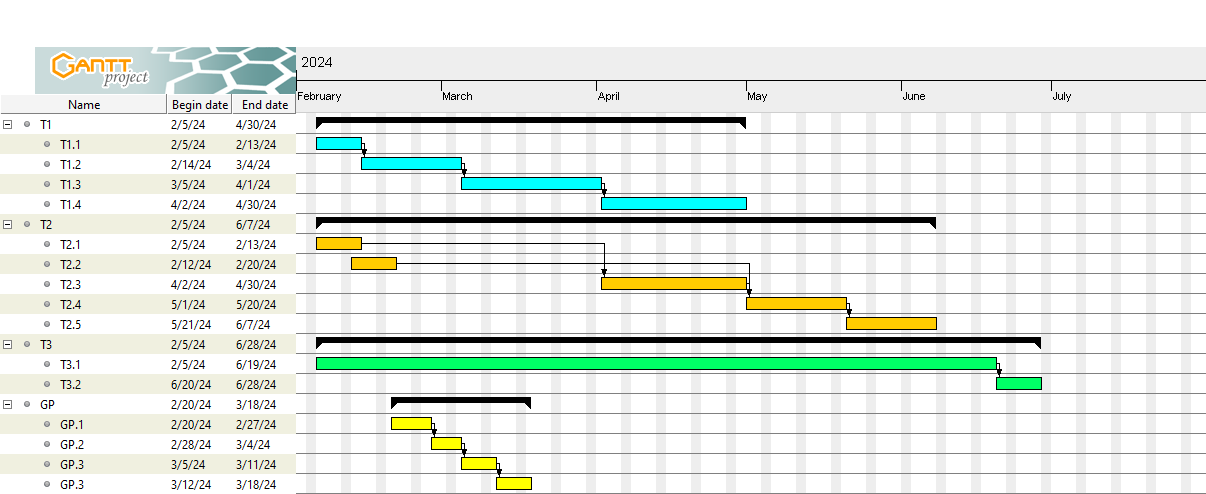
\includegraphics[width=15cm]{img/misc/gantt.png}
    \caption{Diagrama de Gantt, els noms de les tasques fan referència als IDs de la taula resum \ref{taula}. Font: elaboració pròpia.}
    \label{fig:enter-label}
\end{figure}

\newpage

\section{Gestió de riscs}

Com a qualsevol projecte, es poden presentar diferents problemes que poden afectar els resultats obtinguts. A continuació s'analitzaran els més probables i es donarà una possible solució per tal que afectin en la menor mesura al resultat del treball.

\subsection{Termini del projecte}

Un dels problemes principals que es poden tenir durant el projecte és no poder complir tots els objectius plantejats abans del termini d'entrega del TFG.

\begin{itemize}
    \item Impacte: Alt
    \item Solució alternativa: Realitzar una bona planificació temporal abans de començar les tasques principals i fer reunions setmanals amb els directors per tal que em guiïn si em quedo encallat. Si fins i tot amb això no es pot arribar a completar tots els objectius, és important tenir una bona documentació de tota la feina feta perquè el tribunal la pugui valorar.
\end{itemize}

\subsection{Planificació errònia}

Pot ser que alguna de les tasques s'allargui més del que estava previst a la planificació.

\begin{itemize}
    \item Impacte: Alt
    \item Solució alternativa: Incrementar les hores setmanal dedicades al TFG i reduir el temps dedicat a altres tasques que es vegin que no necessiten tant de temps.
\end{itemize}

\subsection{Falta d'experiència en l'àmbit del projecte}

Tot i que he realitzat l'especialitat de computació i, per tant, he fet l'assignatura de Gràfics que es relaciona directament amb els coneixements bàsics per aquest treball, no he fet cap altre més assignatura dedicada als gràfics.

\begin{itemize}
    \item Impacte: Mitjà
    \item Solució alternativa: Dedicar temps suficient a l'inici del treball a recordar i entendre els conceptes més importants per a aquest treball.
\end{itemize}

\subsection{Problemes informàtics}

Tot i que és poc probable, l'ordinador pot fallar i es poden perdre la documentació i el codi del treball. Els serveis que utilitzo al núvol també poden fallar i no tenir accés a la informació que hi tinc. (p. ex. a l'Overleaf).

\begin{itemize}
    \item Impacte: Mitjà
    \item Solució alternativa: Tenir tots els documents i codi del treball en com a mínim dos dispositius (local o al núvol). Per exemple, en el cas del codi tenir-lo en local i al núvol al GitHub. Si l'ordinador falla podria utilitzar el portàtil.
\end{itemize}

\subsection{Corba d'aprenentatge de Blender}

Blender és un programa molt complet per a modelar models 3D, en tenir tantes funcionalitats pot ser complicat per a mi aprendre a utilitzar-lo de manera eficient.

\begin{itemize}
    \item Impacte: Baix
    \item Solució alternativa: Donar més temps a aprendre a utilitzar el programa, per exemple, afegir unes 10 hores a la tasca per tal de poder consultar més tutorials i documentació.
\end{itemize}


\newpage

\section{Pressupost}

Un dels factors més importants per tal que un projecte pugui tirar endavant és saber de quin pressupost es disposa i com es gestiona. A continuació s'explica en detall el pressupost per aquest projecte.

\subsection{Costos de personal}

El cost més important en aquest projecte són els treballadors. Per tant, primer he de definir els rols involucrats en aquest projecte per tal de definir quin sou els hi correspon. Tot i que en aquest projecte només hi estem involucrats els directors i jo, la feina la podem dividir en els rols següents:

\begin{itemize}
    \item Desenvolupador (D): Responsable d'implementar el codi. 
    \item Gestor de projectes (P): Responsable de planificar el projecte i guiar el seu desenvolupament.
    \item Tester (T): Responsable de validar la feina feta pel desenvolupador.
\end{itemize}

Un cop definits els rols, per tal de saber el cost que tenen necessitem saber el salari mitjà de cadascun d'ells a Barcelona. Per això, he consultat la pàgina web PayScale \cite{payscalePayscaleSalary}, on s'indica el salari brut anual. 

Per tal d'obtenir el salari per hora, he calculat les hores treballades en un any de la manera següent, considerant 25 dies de festa (5 setmanes) i una jornada setmanal de 37,5 hores (7,5 hores diàries):

$$\text{hores anuals} = \text{hores setmanals} * \text{setmanes treballades}= 37,5 * (52 - 5) = 1762,5 h $$

A més s'ha d'afegir el cost de la seguretat social que per aproximar serà un 30\% del salari brut.

\begin{table}[H]
    \centering
    \caption{Taula de sou per hora dels diferents rols. Font: elaboració pròpia.}
    \begin{tabular}{|c|c|c|}
         \hline
         Rol & Sou brut (€/hora) & Sou amb SS (€/hora) \\
         \hline
         \hline
         Desenvolupador Junior & 14,2 \cite{payscaleJuniorSoftware} & 18,46 \\
         Gestor de projectes & 27,75 \cite{payscaleProjectManager} & 36,08 \\
         Tester Junior & 13,38 \cite{payscaleSoftwareTester} & 17,39 \\
         \hline
    \end{tabular}
    \label{tab:souperhora}
\end{table}

A partir de la taula \ref{tab:souperhora} juntament amb la planificació d'hores de les tasques es poden calcular els costos dels recursos humans. Font: elaboració pròpia.

\begin{table}[H]
    \centering
    \addtolength{\leftskip} {-4cm}
    \addtolength{\rightskip}{-2cm}
    \caption{Taula amb el resum de les tasques, la seva duració i el seu cost. Font: elaboració pròpia.}
    \begin{tabular}{|c|c|c|c|c|c|c|}
         \hline
         ID & Tasca & Temps & \multicolumn{3}{c}{Temps per rol} & Cost total amb SS (\texteuro) \\
         & & & D & P & T & \\
         \hline
         \hline
         GP.1 & Definició de l’abast i contextualització & 16h & - & 16h & - & 577,2 \\
         GP.2 & Planificació Temporal & 10h & - & 10h & - & 360,75 \\
         GP.3 & Gestió Econòmica i sostenibilitat & 9h & - & 9h & - & 324,68 \\
         GP.4 & Document final & 40h & - & 40h & - & 1443 \\
         \hline
         \hline
         T1.1 & Llegir l'article i familiaritzar-se amb els conceptes & 20h & 20h & - & - & 369,2 \\
         T1.2 & Implementació de l'algorisme bàsic & 30h & 30h & - & - & 553,8 \\
         T1.3 & Addició de característiques i millora de l'eficiència & 60h & 60h & - & - & 1107,6 \\
         T1.4 & Tests i canvis per millorar la visualització & 40h & - & - & 40h & 695,76 \\
         \hline
         \hline
         T2.1 &  Familiaritzar-se amb els conceptes relacionats amb les textures & 5h & 5h & - & - & 92,3 \\
         T2.2 & Aprendre a utilitzar Blender & 10h & 10h & - & - & 184,6 \\
         T2.3 & Crear una \textit{pipeline} per generar les textures & 140h & 140h & - & - & 2584,4 \\
         T2.4 & Integrar la \textit{pipeline} amb Blender & 20h & 20h & - & - & 369,2 \\
         T2.5 & Aplicar les textures al model & 40h & 40h & - & - & 738,4 \\
         \hline
         \hline
         T3.1 & Documentació & 75h & 40h & 35h & - & 2001,025 \\
         T3.2 & Preparació de la presentació i defensa & 25h & 25h & - & - & 461,5 \\
         \hline
         \hline
         \rowcolor{Gray} \textbf{Total} & & \textbf{540h} & \textbf{390h} & \textbf{110h} & \textbf{40h} & \textbf{11863,8} \\
         \hline
    \end{tabular}
    \label{tab:tasques}
\end{table}

\subsection{Costos materials}

Els costos materials d'aquest projecte són només el cost de la torre que utilitzaré per fer tot el projecte, ja que el programari que utilitzaré és gratuït i de codi obert. Per tal de mesurar el cost de l'ordinador he de calcular quina proporció de la vida útil d'aquest usem. La vida útil de la torre és d'uns 5 anys i en va costar uns 700 \texteuro.

$$\text{Cost d'ús de la torre} = \dfrac{\text{Cost torre}}{\text{Vida útil (h)}} \cdot \text{Hores d'ús} = \dfrac{700}{1762,5 \cdot 5} \cdot 540 = 42.89$$

\subsection{Costos genèrics}

Els costos genèrics són els serveis bàsics que utilitzaré durant la realització del treball com ara l'habitatge, la llum, l'aigua… Pago 450€ aproximadament al mes amb tots els serveis inclosos (internet, electricitat i aigua). Per tant, simplement he de multiplicar els mesos en què treballaré en el projecte:

$$\text{Costos genèrics} = 450 \cdot 5 = 2250$$

\subsection{Contingències}

El treball té associats diferents riscs que poden provocar que el cost del projecte sigui més elevant, ja sigui pel fet que s'allargui en el temps o es requereixin més recursos materials. És per això que afegiré un 15\% de marge a tots els costos.

\begin{table}[H]
    \centering
    \label{tab:my_label}
    \caption{Taula amb els valors de contingència per a cada un dels costos. Font: elaboració pròpia.}
    \begin{tabular}{|c|c|c|}
         \hline
         Recursos & Cost base (\texteuro) & Contingència (\texteuro) \\
         \hline
         \hline
         Humans & 11863,8 & 1779,57 \\
         Materials & 42,89 & 6,58 \\
         Genèrics & 2250 & 337,5 \\
         \hline
         \rowcolor{Gray} \textbf{Total} & \textbf{14156,69} & \textbf{2123,65} \\
         \hline
    \end{tabular}
\end{table}

\subsection{Costos imprevistos}

Pel que fa als riscos definits en l'entrega anterior he de definir quin cost poden a arribar a tenir d'acord amb la probabilitat que passin. 

\begin{table}[H]
    \centering
    \label{tab:my_label}
    \caption{Possibles costs associats als riscos. Font: elaboració pròpia.}
    \begin{tabular}{|c|c|c|c|}
         \hline
         Incident & Cost estimat (\texteuro) & Risc & Cost (\texteuro) \\
         \hline
         \hline
         Falta d'experiència en l'àmbit del projecte (15h) & 300 & 50\% & 150 \\
         Planificació errònia (30h) & 500 & 50\% & 250 \\
         Problemes informàtics & 400 & 10\% & 40 \\
         \hline
         \rowcolor{Gray} \textbf{Total} & & & \textbf{440} \\
         \hline
    \end{tabular}
\end{table}

\subsection{Pressupost final}

Per obtenir el pressupost total simplement s'han de sumar tots els costos que he enumerat en les seccions anteriors.

\begin{table}[H]
    \centering
    \caption{Pressupost complet. Font: elaboració pròpia.}
    \label{tab:my_label}
    \begin{tabular}{|c|c|}
    \hline
         Tipus & Cost (\texteuro) \\
         \hline
         \hline
         Recursos humans & 11863,8 \\
         Recursos materials & 42,89 \\
         Recursos genèrics & 2250 \\
         Contingència & 2123,65 \\
         Costos imprevistos & 440 \\
         \hline
         \rowcolor{Gray} \textbf{Total} & \textbf{16720,34} \\
         \hline
    \end{tabular}
\end{table}

\subsection{Control de gestió}

Per tal de poder actuar i evitar els riscs del projecte, seguiré el control de pressupost cada cop que acabi una tasca. Els indicadors que faré servir són:

\begin{itemize}
    \item Desviació del cost: Diferència entre el cost real amb el cost estimat de la taula \ref{tab:tasques}.
    \item Desviació de les hores: Diferència entre el temps dedicat amb el temps previst, també a la taula \ref{tab:tasques}.
\end{itemize}

Amb aquests indicadors puc fer un seguiment precís de si m'estic desviant molt o no de la planificació.

\newpage

\section{Sostenibilitat}

\subsection{Autoavaluació}

Durant els últims anys la sostenibilitat ha pres un paper més important en tots els aspectes de la nostra vida diària, la universitat no n'és una excepció. Durant la carrera en diferents assignatures se'ns ha intentat fer veure la importància de com es treballa en un projecte per fer-lo més sostenible. Des de reciclar maquinari que potser no és útil per al que es feia servir fins ara, però que per altres aplicacions és perfectament vàlid, fins a dissenyar algorismes més eficients tant en temps com en memòria per reduir el temps d'execució i per extensió el seu consum.

A més en els últims anys he començat a veure els efectes que està tenint el canvi climàtic en el món, i a Catalunya en concret, amb temperatures més altes i menys precipitacions. Aquest fet em fa veure que la sostenibilitat està més que justificada i que és un factor molt important a tenir en compte per aquest projecte, però també en els projectes en els quals treballi en el futur.

L'impacte que tindrà aquest projecte en el medi ambient potser serà molt reduït, però reflexionar en cada un dels aspectes de la sostenibilitat serà útil en projectes en els quals treballi amb moltes més persones, utilitzant no només el meu ordinador, sinó centenars, a més de servidors web, superordinadors…

\subsection{Dimensió Econòmica}

\subsubsection{Respecte al Projecte posat en producció (PPP): Reflexió sobre el cost que has estimat per la realització del projecte?}

L'estimació econòmica que he fet pel projecte crec que és bastant acurada, ja que he detallat d'on venen els diferents costos. M'ha sorprès, pel fet que és un treball de la universitat, el cost que tindria realment si es fes en una empresa o en una universitat en un projecte de recerca.

\subsubsection{Respecte a la Vida Útil: Com es resolen actualment els aspectes de costos del problema que vols abordar (estat de l’art)?}

El projecte no requereix molts costos, ja que només és necessari un ordinador amb mínima potència gràfica i, per tant, no és un tema que es tracti en els articles relacionats.

\subsubsection{En què millorarà econòmicament (costos…) la teva solució respecte a les existents?}

Ja que auqest projecte no planteja problemes econòmics la meva solució no en millorarà.

\subsection{Dimensió Ambiental}

\subsubsection{Respecte al Projecte posat en producció (PPP): ¿Has estimat l'impacte ambiental que tindrà la realització del projecte?}

L'impacte ambiental del projecte no és molt elevat, ja que l'energia que faré servir prové de les plaques solars que tinc instalades a casa i com que el recurs principal que utilitzaré és l'electricitat serà molt baix. A més no he hagut de comprar cap component de l'ordinador, que hauria suposat un impacte en el medi.

\subsubsection{Respecte al Projecte posat en producció (PPP): T’has plantejat minimitzar-ne l'impacte, per exemple, reutilitzant recursos?}

Tal com he dit l'energia que usaré és neta i, per tant, és complicat reduir-ne l'impacte.

\subsubsection{Respecte a la Vida Útil: Com es resol actualment el problema que vols abordar (estat de l’art)?, i. ¿En què millorarà ambientalment la teva solució respecte a les existents?}

En el que pot millorar ambientalment la solució que proposi és l'eficiència d'aquesta. És a dir reduïr el màxim el temps dedicat a la generació i visualització dels líquens per no afegir costs energètics als models d'herència cultural.

\subsection{Dimensió Social}

\subsubsection{Respecte al Projecte posat en producció (PPP): Què creus que t’aportarà en l'àmbit personal la realització d’aquest projecte?}

El projecte m'ajudarà a aprendre com gestionar i formar part d'un projecte de cara al futur laboral o acadèmic. A més, crec que aprendre molt sobre gràfics i algorismia, cosa que m'ajudarà a decidir el meu futur, sigui decidir quin màster faré o a quina feina vull aplicar.

\subsubsection{Respecte a la Vida Útil: Com es resol actualment el problema que vols abordar (estat de l’art)? i. ¿En què millorarà socialment (qualitat de vida) la teva solució respecte a les existents?}

La meva solució ajudarà a dotar de realisme a models de monuments importants per la nostra cultura. Cosa que permetrà preservar millor aquests monuments i fer més atractiva la visita virtual d'aquests.

\subsubsection{Respecte a la Vida Útil: Existeix una necessitat real del projecte?}

El projecte no és estrictament necessari per preservar els monuments, però tal com  he dit en la resposta anterior la meva solució fa més atractiu de cara al públic general i millora l'acuracitat dels models.

\newpage

\section{Generació de líquens}

El primer pas per tal de generar líquens realistes és simular el seu creixement i obtenir la forma final per després poder-la texturar. En el meu que cas he decidit utilitzar una variació de l'algorisme anomenat \textit{Diffusion Limited Aggregation} (DLA).

\subsection{Algorisme}

 L'algorisme bàsic de DLA és un model estocàstic utilitzat per simular la formació d'estructures fractals i patrons agregatius. Consisteix en la creació d'un clúster de partícules que creix a mesura que les noves partícules es mouen aleatòriament (difonen) i s'adhereixen al clúster principal quan el toquen (vegeu el pseudocodi \ref{alg:dla}). 

\begin{algorithm}[H]
\caption{Esquema bàsic de l'algorisme DLA}
\begin{algorithmic}[1]
\Procedure{DLA}{n}
\State clúster $\gets \{\{0, 0\}\}$
\For{$i \in \{1,2,...,n\}$}
    \State partícula $\gets$ coordenada aleatòria
    \While{partícula no està en contacte amb el clúster}
        \State partícula $\gets$ mou la partícula en una direcció aleatòria
    \EndWhile
    \State clúster $\gets$ clúster $\cup$ partícula
\EndFor
\State \Return clúster
\EndProcedure
\end{algorithmic}
\label{alg:dla}
\end{algorithm}

 L'algorisme proposat per Desbenoit et al. \cite{Simulating-and-modeling-lichen-growth} l'Open DLA difereix amb el DLA original per com es generen les partícules noves i com aquestes s'agreguen al clúster. Els avantatges de l'Open DLA són la seva eficiència en generar partícules noves i l'addició de paràmetres per tal de modificar la forma final dels líquens, podeu veure la idea bàsica de l'algorisme al pseudocodi \ref{alg-open-dla}. A continuació explicaré els dos passos principals de l'algorisme amb més detall: el moviment i l'agregació.

\begin{algorithm}[H]
\caption{Esquema bàsic de l'algorisme Open DLA}
\begin{algorithmic}[1]
\Procedure{probabitatAgregació}{partícula}
    \State \Return probabilitat de la partícula a agregar-se amb el clúster
\EndProcedure
\Procedure{DLA}{n}
\State C $\gets \{\{0, 0\}\}$ \Comment{$C$ és el clúster}
\For{$i \in \{1,2,...,n\}$}
    \State $p$ $\gets$ coordenada aleatòria
    \While{$p$ no s'ha agregat amb $C$}
        \State $p$ $\gets$ mou la partícula en una direcció aleatòria
        \If{$p$ es mou a més de distància $d$ de $C$}
            \State $p$ $\gets$ coordenada aleatòria dins un radi $r$ de $C$
        \EndIf

        \If{$p$ contacta amb $C$}
            \State rand $\overset{{\scriptscriptstyle\$}}{\leftarrow} [0, 1]$
            \If{probabitatAgregació($p$) $\leq$ rand}
                \State $C$ $\gets$ $C$ $\cup$ $p$ \Comment{Agregació}
            \Else
                \State $p$ $\gets$ coordenada aleatòria dins un radi $r$ de $C$
            \EndIf
        \EndIf
    \EndWhile
\EndFor
\State \Return $C$
\EndProcedure
\end{algorithmic}
\label{alg-open-dla}
\end{algorithm}
 
\subsubsection{Generació i moviment de partícules}

L'article \textit{Simulating and modeling lichen growth} \cite{Simulating-and-modeling-lichen-growth} proposa una manera més eficient de generar les noves partícules respecte a la implementació original del DLA (vegeu la imatge \ref{fig:dla-movement}). Consisteix en primer seleccionar aleatòriament una partícula que ja formi part del clúster i a una distància $r$ d'aquesta generar la nova partícula. La distància $d$ que proposa l'article és $2r + r/2$, on $r$ és el radi del cercle que forma una partícula.

\begin{figure}[H]
    \centering
    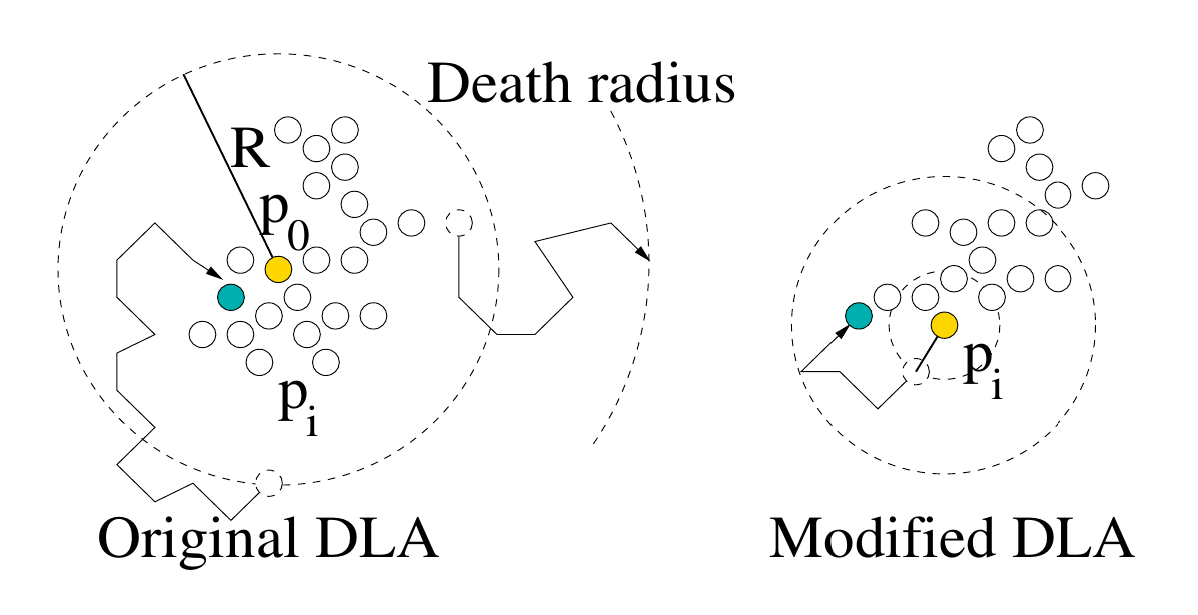
\includegraphics[width=0.6\linewidth]{img/dla/movement.png}
    \caption{Generació i moviment de les partícules en la implementació original i la proposada per Desbenoit et al. \cite{Simulating-and-modeling-lichen-growth}. Font: \textit{Simulating and modeling lichen growth} \cite{Simulating-and-modeling-lichen-growth}.}
    \label{fig:dla-movement}
\end{figure}

En implementar aquesta generació de partícules modificada, no vaig obtenir resultats gaire satisfactoris, ja que les formes que genera són molt compactes.
Finalment, vaig decidir implementar una solució diferent que consisteix a crear les partícules al cercle contenidor centrat en el centre del clúster i amb un radi igual a la distància entre el centre i la partícula més llunyana del clúster. El \textit{death radius} (distància a la qual si arriba una partícula se'n genera una de nova) que he utilitzat és d'un 10 \% més gran que el cicle contenidor. Amb aquesta solució genera formes correctes i millora el rendiment respecte a la implementació original del DLA en què les partícules es generen en una posició aleatòria sense màxim de distància.

Pel que fa al moviment en la meva implementació, les partícules es mouen en una direcció aleatòria, és a dir, a un angle entre $0$ i $2\pi$ radians a una distància igual al radi de les partícules. 

\subsubsection{Agregació}

En el cas de l'algorisme original de DLA, quan una partícula nova entra en contacte amb el clúster s'agrega directament, cosa que no ens permet parametritzar el creixement del liquen i en conseqüència la seva forma final. És per això que l'article \textit{Simulating and modeling lichen growth} \cite{Simulating-and-modeling-lichen-growth} proposa una fórmula amb diferents paràmetres per calcular la probabilitat d'agregar-se amb el clúster.

$$A(p) = \alpha + (1 - \alpha) e ^ {- \sigma (n(p) - \tau) ^ 2} $$

on $n$ és una funció que donada un punt retorna el nombre de partícules agregades en un radi $r \cdot p$ ($r$ és el radi de les partícules) de la partícula a agregar.

Els paràmetres $\alpha$, $\sigma$, $\tau$ i $p$ defineixen la forma final del clúster tal com es veu a la secció de següent.

\subsection{Anàlisi dels resultats parcials}

Per tal de poder veure els efectes dels diferents paràmetres en la forma final del liquen he generat un mateix nombre de partícules modificant un únic paràmetre.

\begin{itemize}
    \item En augmentar el factor $p$ genera líquens amb branques més fines.
    \begin{figure}[H]
         \centering
         \begin{subfigure}[b]{0.3\textwidth}
             \centering
            \includegraphics[width=\textwidth]{img/dla/tests/p/dla_1.500000_0.300000_0.001000_4.000000/color_color_map.png}
            \caption{$p = 1.5$. Font: elaboració pròpia.}
             \label{fig:three sin x}
         \end{subfigure}
         \hfill
         \begin{subfigure}[b]{0.3\textwidth}
             \centering
             \includegraphics[width=\textwidth]{img/dla/tests/p/dla_2.000000_0.300000_0.001000_4.000000/color_color_map.png}
             \caption{$p = 2$. Font: elaboració pròpia.}
             \label{fig:five over x}
         \end{subfigure}
         \hfill
         \begin{subfigure}[b]{0.3\textwidth}
             \centering
             \includegraphics[width=\textwidth]{img/dla/tests/p/dla_2.500000_0.300000_0.001000_4.000000/color_color_map.png}
             \caption{$p = 2.5$. Font: elaboració pròpia.}
             \label{fig:five over x}
         \end{subfigure}
        \label{fig:three graphs}
    \end{figure}
    \item El factor $\tau$ com més elevat és el seu valor més densos és la forma final.
    \begin{figure}[H]
         \centering
         \hfill
         \begin{subfigure}[b]{0.3\textwidth}
             \centering
            \includegraphics[width=\textwidth]{img/dla/tests/tau/dla_2.000000_3.000000_0.001000_2.000000/color_color_map.png}
            \caption{$\tau = 2$. Font: elaboració pròpia.}
             \label{fig:three sin x}
         \end{subfigure}
         \hfill
         \begin{subfigure}[b]{0.3\textwidth}
             \centering
             \includegraphics[width=\textwidth]{img/dla/tests/tau/dla_2.000000_3.000000_0.001000_6.000000/color_color_map.png}
             \caption{$\tau = 6$. Font: elaboració pròpia.}
             \label{fig:five over x}
         \end{subfigure}
         \hfill
        \label{fig:three graphs}
    \end{figure}
    \item El factor $\sigma$ té un efecte en la forma de creixement del liquen com més elevat és el seu valor les branques creixen a totes les direccions a una mida similar.
    \begin{figure}[H]
         \centering
         \begin{subfigure}[b]{0.3\textwidth}
             \centering
            \includegraphics[width=\textwidth]{img/dla/tests/sigma/dla_2.000000_0.300000_0.001000_4.000000/color_color_map.png}
            \caption{$\sigma = 0.3$. Font: elaboració pròpia.}
             \label{fig:three sin x}
         \end{subfigure}
         \hfill
         \begin{subfigure}[b]{0.3\textwidth}
             \centering
             \includegraphics[width=\textwidth]{img/dla/tests/sigma/dla_2.000000_3.000000_0.001000_4.000000/color_color_map.png}
             \caption{$\sigma = 3$. Font: elaboració pròpia.}
             \label{fig:five over x}
         \end{subfigure}
         \hfill
         \begin{subfigure}[b]{0.3\textwidth}
             \centering
             \includegraphics[width=\textwidth]{img/dla/tests/sigma/dla_2.000000_30.000000_0.001000_4.000000/color_color_map.png}
             \caption{$\sigma = 30$. Font: elaboració pròpia.}
             \label{fig:five over x}
         \end{subfigure}
        \label{fig:three graphs}
    \end{figure}
    \item El factor $\alpha$ serveix per inhibir els efectes de la resta de paràmetres, ja que dona una probabilitat per defecte tal com es veu a la fórmula.
    \begin{figure}[H]
         \centering
         \begin{subfigure}[b]{0.3\textwidth}
             \centering
            \includegraphics[width=\textwidth]{img/dla/tests/alpha/dla_2.000000_3.000000_0.001000_4.000000/color_color_map.png}
            \caption{$\alpha = 0.001$. Font: elaboració pròpia.}
             \label{fig:three sin x}
         \end{subfigure}
         \hfill
         \begin{subfigure}[b]{0.3\textwidth}
             \centering
             \includegraphics[width=\textwidth]{img/dla/tests/alpha/dla_2.000000_3.000000_0.010000_4.000000/color_color_map.png}
             \caption{$\alpha = 0.01$. Font: elaboració pròpia.}
             \label{fig:five over x}
         \end{subfigure}
         \hfill
         \begin{subfigure}[b]{0.3\textwidth}
             \centering
             \includegraphics[width=\textwidth]{img/dla/tests/alpha/dla_2.000000_3.000000_0.100000_4.000000/color_color_map.png}
             \caption{$\alpha = 0.1$. Font: elaboració pròpia.}
             \label{fig:five over x}
         \end{subfigure}
        \label{fig:three graphs}
    \end{figure}
\end{itemize}


\newpage

\section{Subdivisió de liquens}

Un cop s'ha generat la forma del liquen el següent pas és la subdivisió d'aquest en clústers per tal poder texturar-los amb una textura amb una forma arbitrària, ja que és molt complicat aplicar una sola textura a tot el liquen perquè quedaria massa deformada. L'algorisme que he escollit per la subdivisió de clústers és el KMeans, aquest algorisme té dos procediments principals: el càlcul dels centroides dels clústers i el càlcul dels clústers a partir dels centroides (vegeu el pseudocodi \ref{alg:kmeans}).

\begin{algorithm}[H]
\caption{Esquema senzill de l'algorisme KMeans}
\begin{algorithmic}[1]
\Procedure{KMeans}{k}
\State centroides $\gets k$ coordenades aleatòries
\State clústers $\gets$ calcula els clústers a partir dels centroides
\State nousCentroides $\gets$ calcula els nous centroides a partir dels clusters
\While{nousCentroides $\neq$ centroides}
    \State centroides $\gets$ nouCentroides
    \State clústers $\gets$ calcula els clústers a partir dels centroides
    \State nousCentroides $\gets$ calcula els nous centroides a partir dels clusters
\EndWhile
\State \Return clústers
\EndProcedure
\end{algorithmic}
\label{alg:kmeans}
\end{algorithm}

A continuació, explicaré l'evolució de la meva implementació i les modificacions que he fet a l'algorisme original per tal de satisfer certes restriccions que han de tenir els clústers, com ara la seva circularitat i connectivitat.

\subsection{Expansió dels clústers}

Un dels passos de l'algorisme KMeans és l'assignació de les partícules als diferents clústers, que en el cas de la meva implementació és una expansió. A continuació explicaré les diferents tècniques que he implementat, els seus avantatges i inconvenients.

\subsubsection{KMeans original}
És la implementació més senzilla de l'algorisme KMeans, en aquest cas els clústers no s'expandeixen, ja que per saber a quin clúster pertany cada punt es fa servir la distància entre el punt i el centroide del clúster corresponent. Aquesta implementació té problemes molt obvis quan es fa una visualització:
\begin{itemize}
    \item Els clústers creixen per l'espai buit, ja que s'utilitza la distància euclidiana per agregar les partícules als clústers (la imatge \ref{fig:espai-buit}).
    \begin{figure}[H]
        \centering
        
\includegraphics[width=0.5\linewidth]{img/kmeans/first/example.png}
        \caption{Exemple d'un clúster (color lila) expandint-se en espai buit.}
        \label{fig:espai-buit}
    \end{figure}
\end{itemize}

\subsubsection{KMeans amb expansió simple}
Per tal d'evitar que els clústers s'expandeixin sense continuïtat, vaig decidir utilitzar un \textit{Breadth-first search} (BFS) des de cada un dels centroides. L'expansió és simple, ja que el BFS  s'expandeix només en les direccions de veïnatge de von Neumann (amunt, avall, a la dreta i a l'esquerra) i, per tant, no es necessita una cua de prioritat perquè totes les arestes tenen distància 1, que és el mateix a no tenir pesos.
\begin{itemize}
    \item Els clústers creen fronteres amb dents de serra i s'expandeixen no uniformement, ja que no hi ha prioritat per al centroide més proper (vegeu les imatges \ref{fig:serra} i \ref{fig:recte}).
    \begin{figure}[H]
        \centering
        
\includegraphics[width=0.5\linewidth]{img/kmeans/second/example.png}
        \caption{Exemple en el qual el clúster de color verd més clar ha bloquejat el creixement dels altres clústers.}
        \label{fig:serra}
    \end{figure}
    \begin{figure}[H]
        \centering
        
\includegraphics[width=0.5\linewidth]{img/kmeans/second/example_2.png}
        \caption{Exemple en el qual es creen fronteres massa rectes.}
        \label{fig:recte}
    \end{figure}
\end{itemize}

\subsubsection{KMeans amb cua de prioritat i expansió en diagonal \label{subsec:expansio-prioritat}}

Aquesta implementació difereix amb l'anterior amb què les partícules es poden expandir cap a totes les partícules del voltant, és a dir en les direccions de veïnatge de Moore. En aquest cas es necessita una cua de prioritat perquè  les arestes que connecten els punts del liquen ja no tenen els mateixos pesos: la diagonal tindrà un pes de $\sqrt{2}$. Per tal d'entendre millor com s'expandeixen els clústers he generat la imatge \ref{fig:cluster-expansio} on s'expandeix un dels clústers.

Un altre factor important és que els clústers creixen en paral·lel és per això que han de créixer d'una manera justa. Un clúster no creix de manera justa quan té menys punts a la cua de prioritat que la resta, que es pot donar per al lloc on es trobi del liquen, i comença a agregar punts que per distància li correspondrien a un altre clúster. És per això que en l'algorisme que proposem, els clústers es poden expandir a una distància màxima a cada iteració i aquesta distància s'incrementa en una unitat en cada iteració perquè és la distància mínima de les arestes. En la imatge \ref{fig:clusters-expansio} es pot veure aquesta expansió en paral·lel.

% \begin{algorithm}[H]
% \caption{Esquema bàsic de l'algorisme d'expansió.}
% \begin{algorithmic}[1]
% \Procedure{assignaClusters}{$k$}
% \State $C$ $\gets$ llista de mida $k$ buida \Comment{Clústers}
% \State $c$ $\gets$ $k$ centroides dels $C$ anteriors
% \State $Q$ $\gets$ llista de mida $k$ amb cues de prioritat amb els $c$ i distància 0
% \State $D$ $\gets$ 1 \Comment{Distància màxima d'expansió dels $C$}
% \State cuesBuides $\gets$ fals
% \While{not cuesBuides}
%     \For{i $\in$ 0..k}
%         \State $p, d \gets Q_i.pop()$ \Comment{p és un punt i $d$ la distància d $p$ al centroide}
%         \If{$d > D$}
%             \State break
%         \EndIf
%         \If{$p$ no ha estat visitat}
%             \State $C_i \gets C_i \cup p$
%             \State $v, d_p \gets$ veïns de $p$ i la seva distància a $p$ 
%             \State $Q_i.push(v, d_v + d)$
%             \State marca $p$ com a visitat
%         \EndIf
%     \EndFor
%     \State $D \gets D + 1$
%     \State cuesBuides $\gets$ cert si totes les cues de $Q$ estan buides
% \EndWhile
% \State \Return $C$
% \EndProcedure
% \end{algorithmic}
% \end{algorithm}

\begin{figure}[H]
    \centering
    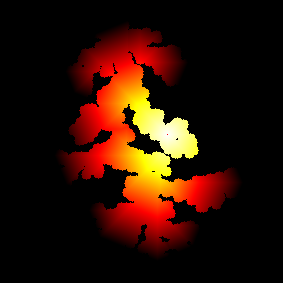
\includegraphics[width=0.4\linewidth]{img/kmeans/heatmap.png}
    \caption{Exemple d'expansió d'un dels clústers mitjançant BFS amb una cua de prioritat, com més lluny del centroide el color és més fosc. Font: elaboració pròpia.}
    \label{fig:cluster-expansio}
\end{figure}

\begin{figure}[H]
    \centering
    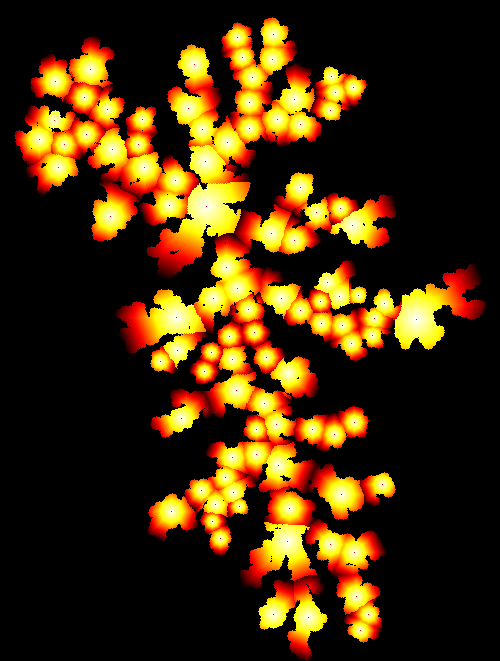
\includegraphics[width=0.5\linewidth]{img/kmeans/heatmap_2.png}
    \caption{Exemple d'un liquen dividit en diferents clústers i la seva expansió, on el color més clar indica proximitat al centroide i color més fosc més distància. Font: elaboració pròpia.}
    \label{fig:enter-label}
    \label{fig:clusters-expansio}
\end{figure}

\subsection{Càlcul dels centroides \label{subsec:centroides}}

L'altre pas important de l'algorisme KMeans és el càlcul dels centroides a partir dels clústers actuals per tal de poder executar la següent iteració. En el cas de l'algorisme de KMeans original és molt senzill, ja que simplement s'agafa el punt mitjà aritmètic de tots els punts d'un clúster.

Però en el cas de la versió que usa BFS ja no es pot utilitzar aquest mètode, ja que el punt mitjà pot quedar fora de l'àrea del liquen si aquest és convex, cosa que després no permetria expandir el BFS. Per tal d'obtenir un centroide vàlid he decidit calcular el punt més intern del clúster, és a dir, aquell punt pertanyent al clúster pel qual la seva distància mínima al perímetre del clúster és la més gran.

\subsection{Circularitat}

Ja que és preferible que els clústers siguin aproximadament circulars per facilitar la parametrització de la textura, he afegit una mesura de circularitat dels clústers. La circularitat es pot definir com la ràtio entre l'àrea d'un clúster, i l'àrea del cercle que tindria el mateix perímetre que el clúster:

$$c_i = 4 * \pi * \frac{a_i}{p_i^2}$$

on $a_i$ és l'àrea del clúster i $p_i$ el perímetre del clúster. El valor que retorna és entre 0 i 1, com més gran més circular.

\subsubsection{Flood filling \label{subsubsec:flood-filling}}

Tal com es veu a la fórmula anterior, per calcular la circularitat es necessita el perímetre i l'àrea dels clústers. Pel que fa a l'àrea és molt senzill, ja que és igual al nombre de partícules del clúster. En canvi, per calcular el perímetre no tenim un mètode tan directe. Primer de tot, vaig implementar un algorisme molt naïf que iterava tots els punts del clúster i agafava com a perímetre tots aquells que tinguessin contacte amb un punt que no és del clúster. El problema és que és possible que un clúster tingui un forat en el seu interior, cosa que amb aquest algorisme seria detectat com a perímetre exterior. És per això que finalment vaig decidir utilitzar l'algorisme anomenat \textit{Flood filling}, que tal com indica el seu nom consisteix a \textit{inundar} l'àrea exterior del clúster per poder detectar les partícules que fan de perímetre. Per tal de fer-lo més eficient, la \textit{inundació} es fa en un rectangle contenidor que té com a vèrtexs les coordenades mínimes i màximes del clúster.

\subsubsection{Test de circularitat}

A continuació, es pot veure el liquen filtrat per diferents valors de circularitat mínima. Els clústers tenen una circularitat molt baixa en general, on només 5 tenen una circularitat acceptable de 0.7 (vegeu la imatge \ref{fig:0.7-circularuty}). És per això que en l'algorisme final proposem subdividir els clústers menys circulars.

\begin{figure}[H]
     \centering
     \begin{subfigure}[b]{0.3\textwidth}
         \centering
         
\includegraphics[width=\textwidth]{img/kmeans/circularity/0.500000_color_map.png}
         \caption{Clústers amb una ràtio de circularitat $> 0.5$}
         \label{fig:y equals x}
     \end{subfigure}
     \hfill
     \begin{subfigure}[b]{0.3\textwidth}
         \centering
         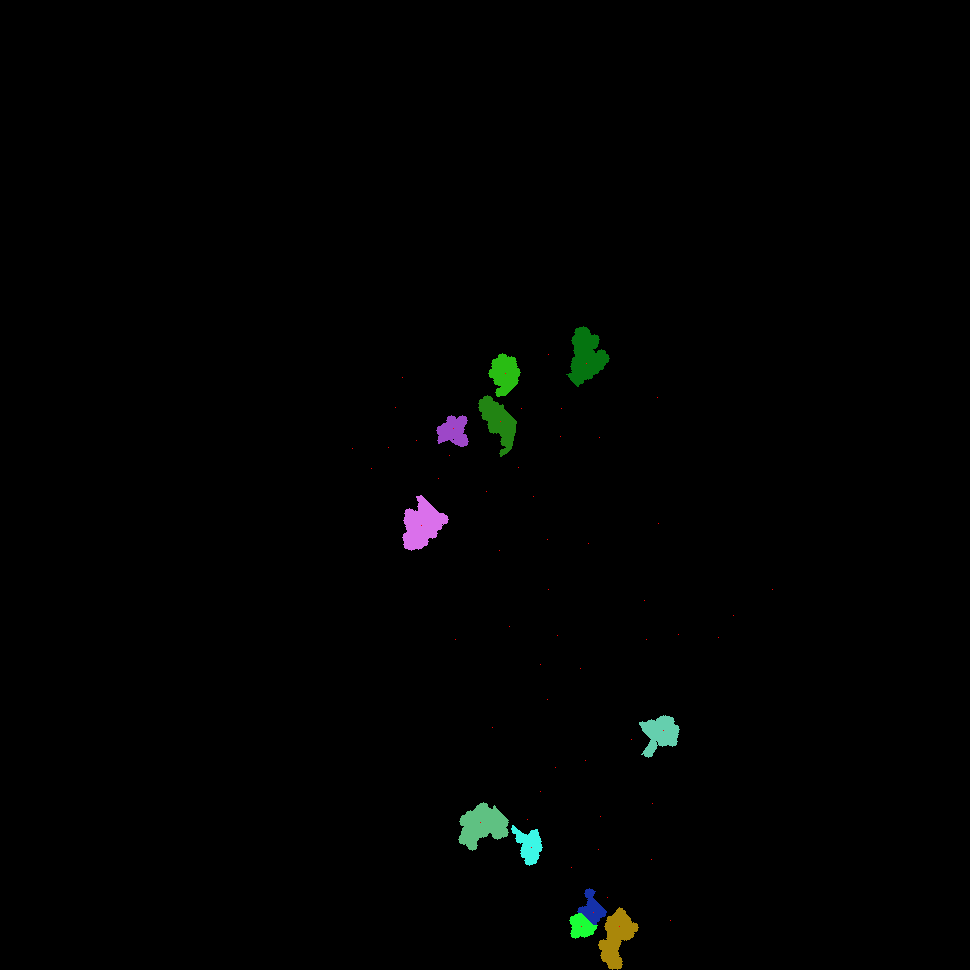
\includegraphics[width=\textwidth]{img/kmeans/circularity/0.600000_color_map.png}
         \caption{Clústers amb una ràtio de circularitat $> 0.6$}
         \label{fig:three sin x}
     \end{subfigure}
     \hfill
     \begin{subfigure}[b]{0.3\textwidth}
         \centering
         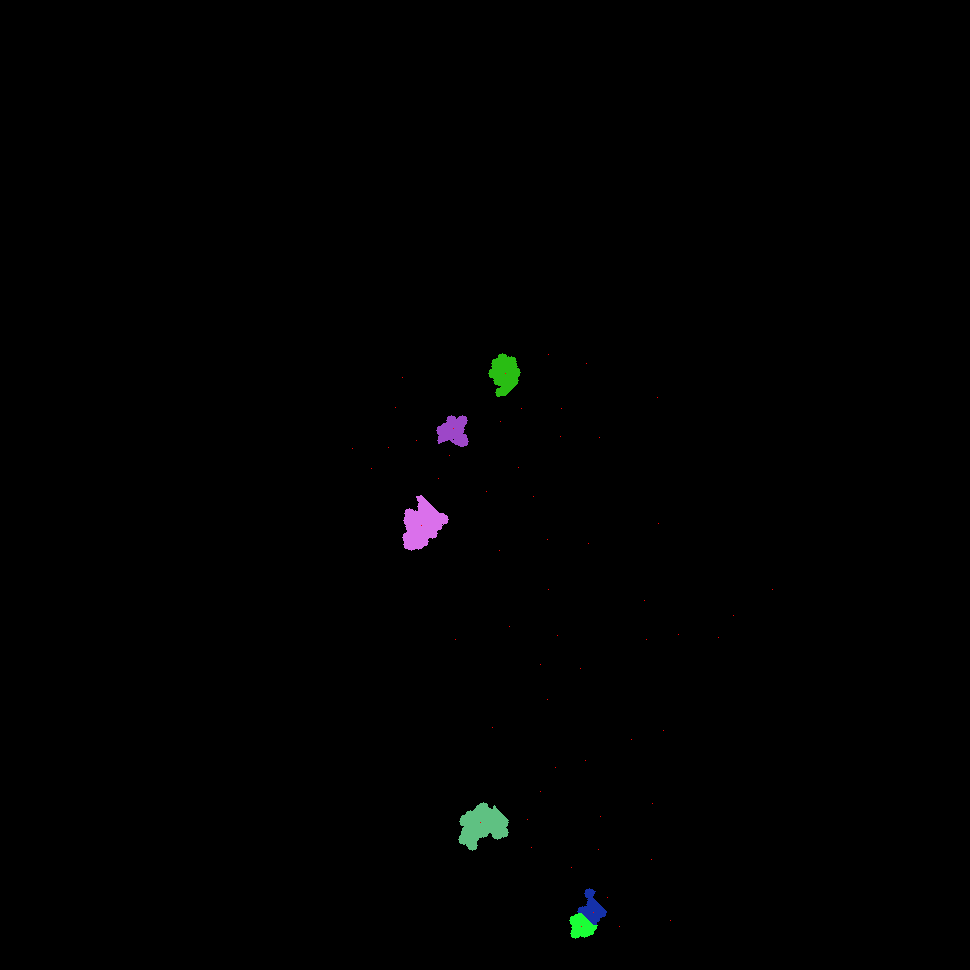
\includegraphics[width=\textwidth]{img/kmeans/circularity/0.700000_color_map.png}
         \caption{Clústers amb una ràtio de circularitat $> 0.7$}
         \label{fig:0.7-circularuty}
     \end{subfigure}
        \caption{Comparació d'un mateix liquen amb clústers amb certa circularitat.}
        \label{fig:circularity-1}
\end{figure}

\subsection{Algorisme final}

La implementació de l'algorisme KMeans que he fet servir per subdividir el liquen utilitza l'expansió amb la cua de prioritat \ref{subsec:expansio-prioritat} i els centroides com el punt més interior \ref{subsec:centroides} (vegeu el pseudocodi d'aquesta implementació \ref{alg:kmeans-final}).

A part de fer servir aquestes modificacions per a obtenir clústers més circulars he seguit la següent estratègia, primer subdividir el liquen en un número no molt elevat de clústers i després subdividir els clústers que no són prou circulars, és a dir, que no superen un mínim de ràtio de circularitat. Si en aquesta subdivisió els clústers resultants no són prou circulars es defineixen els centroides aleatòriament una altra vegada i es repeteix l'algorisme, això es fa un número definit de vegades que no és molt elevat, en el meu cas es prova 5 vegades. Si així i tots els clústers resultants no són prou circulars, ens quedem amb aquests clústers i els subdividim, això sí, només si aquests clústers tenen una mida mínima que definim nosaltres per tal que no siguin massa petits per texturar després.

\begin{algorithm}[H]
\caption{Esquema bàsic de la meva implementació de l'algorisme KMeans, on $k$: nombre de clústers de la primera subdivisió, $P$: conjunt de punts, $c$: circularitat mínima $0 \le c \le 1$ i $m$: mida mínima dels clústers.}
\begin{algorithmic}[1]
\Procedure{KMeans}{$k$, $P$, $c$, $m$}
$C \gets KMeans(k, P)$
\For{$i \in 0..k$}
    \If{circularitat($C_i$) $> c$}
        \State continue
    \EndIf
    \State $nk \gets 2$
    \State $c_i \gets$ fals
    \State $C' \gets$ divisioClusters($nk$, $C_i$)
    \State $c_i \gets \forall_{1 \le j \le nk}$ circularitat($C'_j$) $> c$
    \While{not $c_i \And$ $\forall_{1 \le j \le nk} |C'_j| > m$}
        \State $nk \gets nk + 1$
        \State $C' \gets$ divisioClusters($nk$, $C_i$)
        \State $c_i \gets$ $\forall_{1 \le j \le nk}$ circularitat($C'_j$) $> c$
    \EndWhile
    \State $C \gets C \cup C'$
\EndFor
\State \Return $C$
\EndProcedure
\end{algorithmic}
\label{alg:kmeans-final}
\end{algorithm}

\subsection{Anàlisi dels resultats parcials}

Per tal de poder comprovar realment si aquesta implementació millora els resultats de circularitat he tornat a filtrar els clústers finals per la seva circularitat per poder-ho comparar amb la imatge \ref{fig:circularity-1}. Com es pot comprovar en la imatge \ref{fig:circularity-0.7} hi ha molts més clústers amb una circularitat superior a 0.7. Així i tot, encara hi ha marge de millora, ja que encara hi ha bastants clústers amb una circularitat inferior.

\begin{figure}[H]
     \centering
     \begin{subfigure}[b]{0.3\textwidth}
         \centering
         
\includegraphics[width=\textwidth]{img/kmeans/circularity/first_color_map.png}
         \caption{Primera subdivisió.}
         \label{fig:y equals x}
     \end{subfigure}
     \hfill
     \begin{subfigure}[b]{0.3\textwidth}
         \centering
         
\includegraphics[width=\textwidth]{img/kmeans/circularity/final_color_map.png}
         \caption{Subdivisió final.}
         \label{fig:three sin x}
     \end{subfigure}
     \hfill
     \begin{subfigure}[b]{0.3\textwidth}
         \centering
         
\includegraphics[width=\textwidth]{img/kmeans/circularity/filtered_color_map.png}
         \caption{Clústers amb una ràtio de circularitat $> 0.7$}
         \label{fig:circularity-0.7}
     \end{subfigure}
        \caption{Resultats de la meva implementació de l'algorisme KMeans.}
        \label{fig:three graphs}
\end{figure}

\newpage

\section{Parametrització de textures}

La parametrització de textures consisteix a traduir les coordenades d'una textura, ja sigui de color, normals, desplaçament..., a les coordenades d'un polígon que volem texturar. En aquesta secció explorem diferents maneres de parametritzar els clústers i en discutim els resultats.

\subsection{MVC}

El Mean Value Coordinates (MVC), proposat per Michael S. Floater \cite{FLOATER200319}, és un mètode que permet calcular els pesos que defineixen un punt de l'interior d'un polígon qualsevol a partir dels vèrtexs d'aquest polígon qualsevol sigui còncau o convex (vegeu la imatge \ref{fig:mvc-polygon}), tema rellevant de cara a les següents seccions. És a dir, el punt és igual a la suma d'uns pesos multiplicats pels vèrtexs del polígon.

$$\sum_{i=1}^{k} w_i \cdot v_i = v_0$$

on $k$ és el nombre de vèrtexs del polígon, $v_i$ el vèrtex i-èssim, $w_i$ el pes corresponent al $v_i$ i $v_0$ el punt interior del polígon.

\begin{figure}[H]
    \centering
    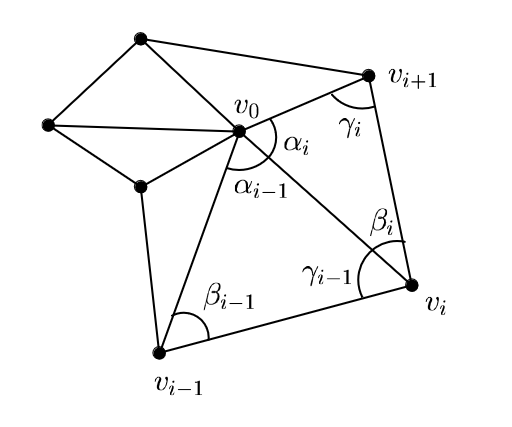
\includegraphics[width=0.5\linewidth]{img/param/mvc.png}
    \caption{Polígon on s'indiquen els angles corresponents als vèrtexs del contorn. On $v_0$ pot ser un punt qualsevol de l'interior del polígon i on $v_>0$ són els vèrtexs del polígon. Font: Michael S. Floater \cite{FLOATER200319}.}
    \label{fig:mvc-polygon}
\end{figure}

Per tal de calcular el valor dels pesos, Michael S. Floater \cite{FLOATER200319}, proposa la següent fórmula dels pesos per a cada un dels vèrtexs de la capsa contenidora:

$$w_i(v_0) = \frac{\tan{\alpha_{i - 1}/2} + \tan{\alpha_{i - 1}/2}}{||v_i - v_0||}$$

on $w_i(v_0)$ és el pes que correspon al vèrtex $v_i$ del polígon i els angles són els definits a la imatge \ref{fig:mvc-polygon}.

El MVC és útil en el meu cas perquè ens permet fer de traductor entre dos polígons. És a dir, si tenim un clúster en el qual he definit $n$ vèrtexs que defineixen el seu contorn (vegeu la imatge \ref{fig:correct-convex-hull}) i una textura en la qual també definim $n$ vèrtexs que defineixin el contorn, podem calcular els pesos d'un punt qualsevol del clúster i a partir dels vèrtexs que he definit de la textura calcular el punt que correspon a la textura.

$$vt_0 = \sum_{i=1}^{n} w_i(vc_0) \cdot vt_i$$

on $vt_0$ és el \textit{target point} de la textura, $w_i(vc_0)$ el pes corresponent al vèrtex $vc_i$ del clúster respecte al punt del clúster $vc_0$ i $vt_i$ el vèrtex i-èssim del polígon que defineix la textura.

Per tal de poder aplicar aquesta fórmula es necessita que els vèrtexs dels dos polígons estiguin ordenats. A més per millorar els resultats i reduir les deformacions, la distància entre $vt_i$-$vt_{i+1}$ i $vc_i$-$vc_{i+1}$ ha de tenir la mateixa proporció en el perímetre dels polígons corresponents. 

A continuació es poden veure els resultats d'aplicar el MVC per tal d'obtenir el color de la textura original, en aquest cas un cercle  (vegeu la imatge \ref{fig:cercle-tex-original}), i aplicar-lo als clústers (vegeu la imatge \ref{fig:mvc-clusters}). Es pot veure que els clústers deformen la textura per adaptar el cercle a la forma que tenen. Per tal de calcular els vèrtexs que formen els polígons de la textura i els clústers per a aquest exemple he utilitzat la tècnica anomenada \textit{convex hull} que explicarem en la següent secció.

\begin{figure}[H]
     \centering
     \begin{subfigure}[b]{0.4\textwidth}
         \centering
         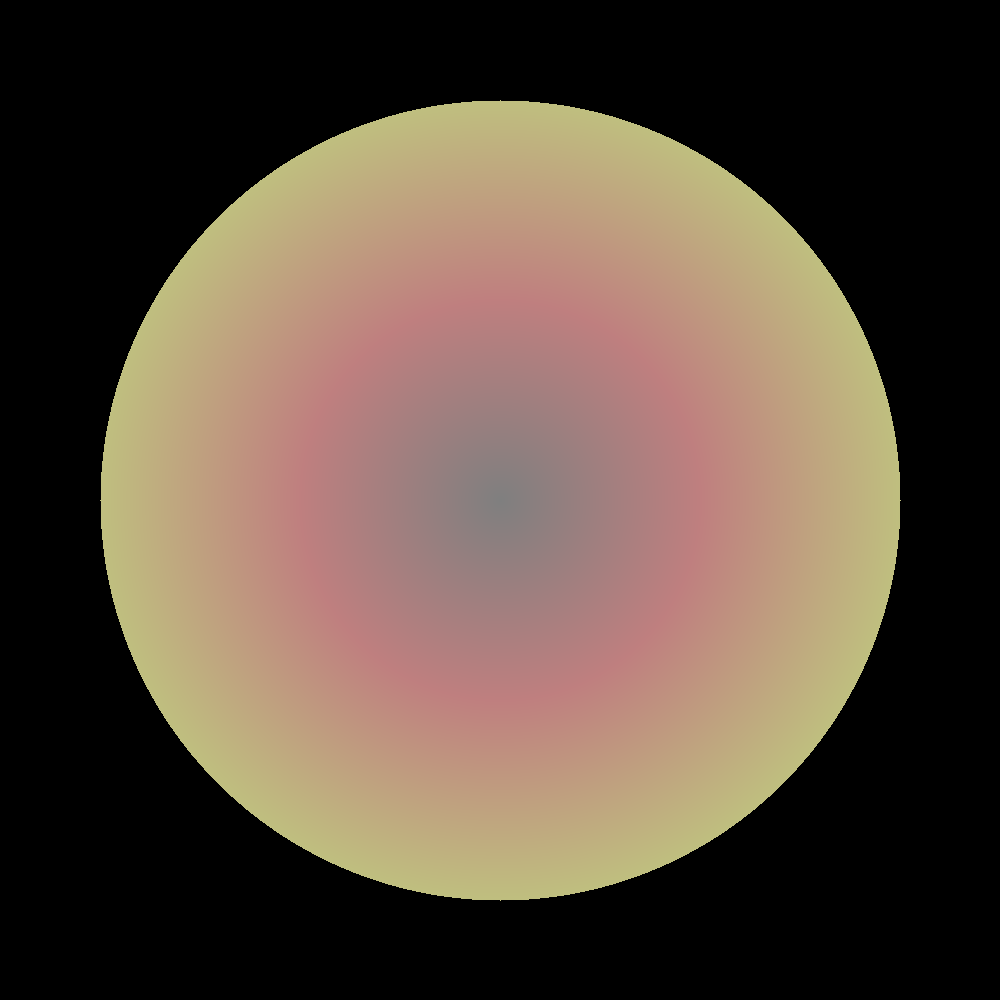
\includegraphics[width=\textwidth]{img/param/circle_normal_map.png}
         \caption{Textura original}
         \label{fig:cercle-tex-original}
     \end{subfigure}
     \hfill
     \begin{subfigure}[b]{0.4\textwidth}
         \centering
         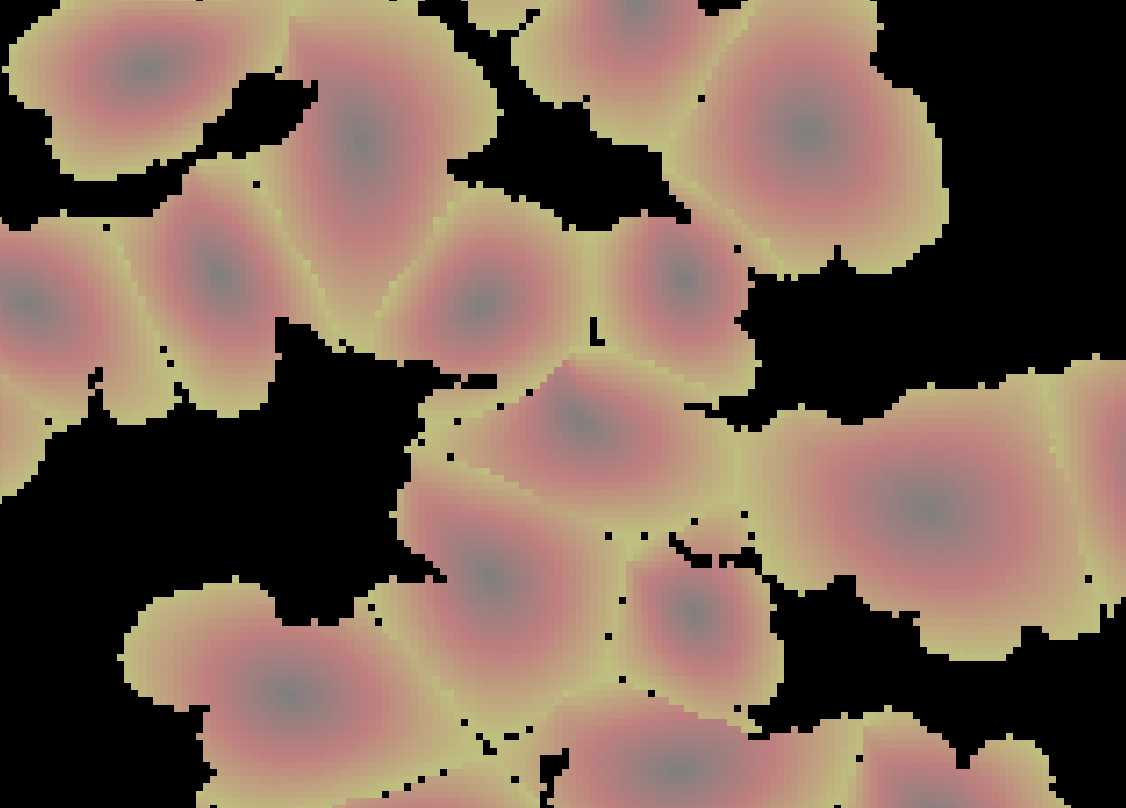
\includegraphics[width=\textwidth]{img/param/circle_param.png}
         \caption{Clústers texturats a partir de la textura original}
         \label{fig:mvc-clusters}
     \end{subfigure}
        \caption{Exemple de la parametrització de la textura original als clústers utilitzant el MVC i el \textit{convex hull} dels clústers.}
        \label{fig:three graphs}
\end{figure}

\newpage

\subsection{Convex Hull}

Una envolupant convexa (\textit{convex hull} en anglès) es defineix com a un subconjunt de punts que defineixen un polígon convex que conté tots el conjunt de punts (vegeu la imatge \ref{fig:convex-hull}). 

\begin{figure}[H]
    \centering
    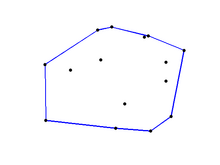
\includegraphics[width=0.6\linewidth]{img/misc/envolupant_convexa.png}
    \caption{Exemple d'un \textit{convex hull}. Font: Viquièdia.}
    \label{fig:convex-hull}
\end{figure}

Un dels algorismes més eficients per calcular el \textit{convex hull} s'anomena Graham Scan proposat per R. L. Graham \cite{GRAHAM1972132} i té una complexitat computacional de $O(n\log{n})$, on $n$ és el nombre de punts. La idea de l'algorisme és bastant senzilla: 

\begin{itemize}
    \item L'algorisme comença trobant el punt amb la coordenada $y$ més petita. Aquest punt es troba sempre al \textit{convex hull}. Aleshores, l'algorisme ordena els punts restants pel seu angle polar respecte al punt inicial.
    \item En el següent pas l'algorisme afegeix punts iterativament al \textit{convex hull}. A cada iteració, l'algorisme comprova si els dos últims punts afegits a la \textit{convex hull} formen un gir a la dreta. Si ho fan, l'últim punt s'elimina de l'envolupant. En cas contrari, el següent punt de la llista ordenada s'afegeix al \textit{hull}.
    \item L'algorisme acaba quan s'han afegit tots els punts al \textit{convex hull}.
\end{itemize}
Els avantatges que té aquest algorisme és que ens retorna els vèrtexs del \textit{convex hull} ordenats, cosa necessària per a utilitzar el MVC. A més, tal com es veu en els resultats en els casos que els clústers no són prou circulars la textura no queda deformada, però sí tallada.

Un dels inconvenients és que l'algorisme retorna el nombre mínim de vèrtexs que creen el \textit{convex hull} i és per això que el nombre de vèrtexs del \textit{convex hull} de la textura original i el \textit{convex hull} del clúster poden diferir i, per tant, el MVC no es pot aplicar. Una solució a aquest problema és crear una textura \textit{proxy} que explicarem a la secció \ref{sec:param-proxy}.

% \begin{algorithm}[H]
% \caption{Graham Scan per al Convex Hull}
% \begin{algorithmic}[1]
% \Procedure{GrahamScan}{$P$}
%     \State $n \gets \text{length}(P)$
%     \If{$n < 3$}
%         \State \Return $P$
%     \EndIf
    
%     \State $P_0 \gets \text{point with lowest y-coordinate (ties are broken by x-coordinate)}$
%     \State $\text{Sort}(P[1:n-1], \text{by polar angle with respect to } P_0)$
%     \State $\text{Push}(P_0, S)$
%     \State $\text{Push}(P[1], S)$

%     \For{$i \gets 2$ \textbf{to} $n-1$}
%         \While{$\text{orientation}(\text{n\_t\_p}(S), \text{top}(S), P[i]) \neq \text{counter-clockwise}$}
%             \State $\text{Pop}(S)$
%         \EndWhile
%         \State $\text{Push}(P[i], S)$
%     \EndFor

%     \State \Return $S$ 
% \EndProcedure

% \Function{orientation}{$p, q, r$}
%     \State $\text{val} \gets (q_y - p_y) \times (r_x - q_x) - (q_x - p_x) \times (r_y - q_y)$
%     \If{$\text{val} = 0$}
%         \State \Return \text{collinear}
%     \ElsIf{$\text{val} > 0$}
%         \State \Return \text{clockwise}
%     \Else
%         \State \Return \text{counter-clockwise}
%     \EndIf
% \EndFunction

% \Function{next\_to\_top}{$S$}
%     \State $\text{top\_element} \gets \text{Pop}(S)$
%     \State $\text{next\_to\_top} \gets \text{top}(S)$
%     \State $\text{Push}(\text{top\_element}, S)$
%     \State \Return $\text{next\_to\_top}$
% \EndFunction

% \end{algorithmic}
% \end{algorithm}

\subsubsection{Anàlisi dels resultats parcials}

En els clústers de la figura \ref{fig:correct-convex-hull} es pot veure que quan el \textit{convex hull} segueix correctament la forma del clúster el resultat de la texturació és proper a la textura original, sense grans deformacions. 

\begin{figure}[H]
    \centering
    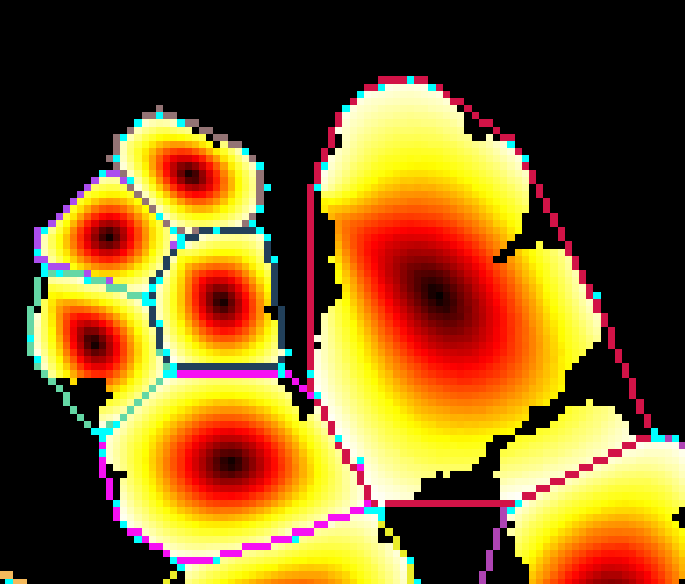
\includegraphics[width=0.5\linewidth]{img/param/conex_hull.png}
    \caption{Exemple dels \textit{convex hull} de diferents clústers. Font: elaboració pròpia.}
    \label{fig:correct-convex-hull}
\end{figure}

En canvi, quan els clústers tenen formes que difereixen molt del seu \textit{convex hull}, com és en el cas de la imatge \ref{fig:ch-deformed}, la textura original queda retallada. Però, en canvi, no queda deformada, fet que depenent del resultat que vulguem pot ser útil.

\begin{figure}[H]
    \centering
    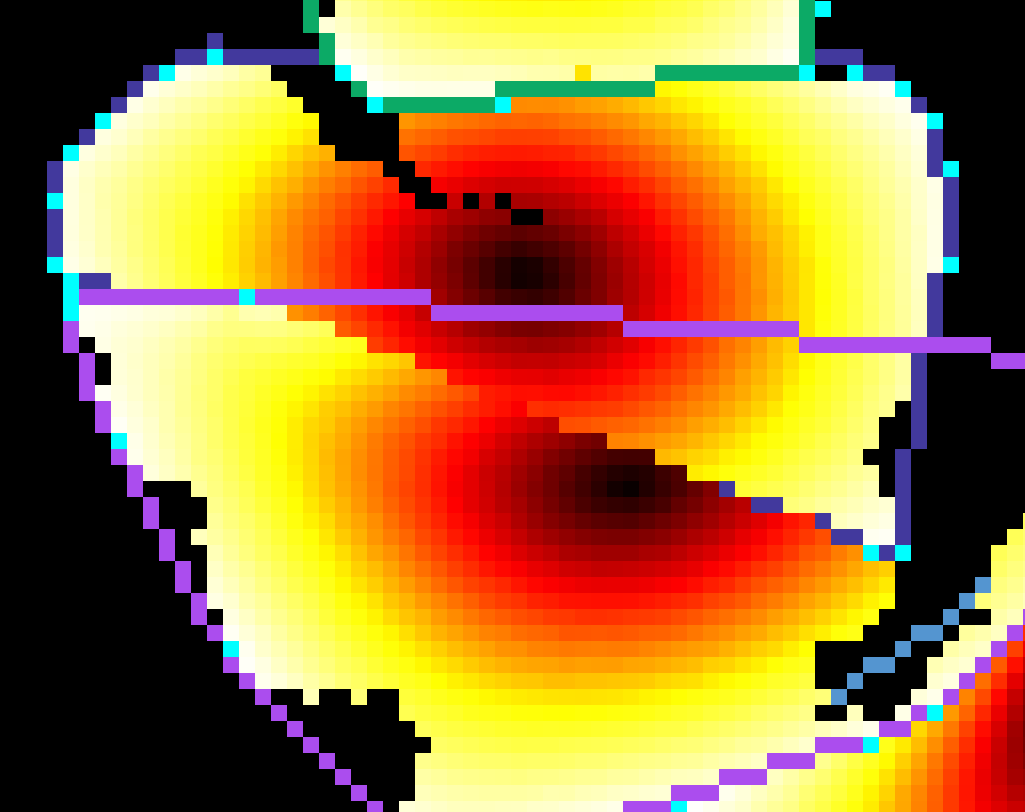
\includegraphics[width=0.5\linewidth]{img/param/cut_texture.png}
    \caption{Exemple on la textura queda tallada per la forma del \textit{convex hull}. Font: elaboració pròpia.}
    \label{fig:ch-deformed}
\end{figure}

\subsection{Concave Hull}

Ja que el \textit{convex hull} en els clústers que no són tan circulars la textura queda tallada, vaig decidir provar d'utilitzar directament el contorn dels clústers com a \textit{hull}. L'anomeno \textit{concave hull} perquè en aquest cas sí que hi pot haver costats de l'envolupant que tenen un angle còncau entre si.

Per tal de poder calcular el contorn dels clústers he utilitzat l'algorisme que ja he descrit a \ref{subsubsec:flood-filling}, anomenat \textit{Flood filling}. Aquest algorisme no retorna els contorns ordenats, és per això que un cop s'obté el contorn s'han de recórrer els punts i ordenar-los. Tot i que aquesta tasca pot semblar trivial, en alguns casos concrets cal tenir una mena de backtracking per a quan es recorren punts en un sortint d'un píxel d'amplada (vegeu la imatge \ref{fig:promunicio}).

\begin{figure}[H]
    \centering
    
\includegraphics[width=0.4\linewidth]{img/param/concave_hull/sortint.png}
    \caption{Exemple en el qual un clúster (turquesa) té un sortint amb un píxel d'amplada. Font: elaboració pròpia.}
    \label{fig:promunicio}
\end{figure}

Per tal que l'algorisme funcioni en aquests casos concrets vaig afegir una pila que conté els punts que s'han visitat anteriorment i que tenen algun camí a recórrer a part de l'actual. Això permet que quan s'arriba a un punt sense cap punt per a on continuar i no sigui el final del contorn, es miri el primer valor de la pila i es continuï el recorregut per aquell punt.

Un cop obtingut el contorn ordenat, s'han de descartar punts d'aquest per tal que el MVC funcioni correctament. Com per exemple agafar un de cada 10 punts consecutius del contorn. L'avantatge d'aquest mètode respecte al \textit{convex hull} és que ens permet definir el nombre de vèrtexs que volem que tingui el \textit{hull}.

\subsubsection{Anàlisi dels resultats parcials}

En general, els resultats de texturació amb el \textit{concave hull} són prou similars als del \textit{convex hull} en els casos que els clústers són circulars, tal i com es pot veure a la imatge \ref{fig:concave-hull-clusters}.

\begin{figure}[H]
    \centering
    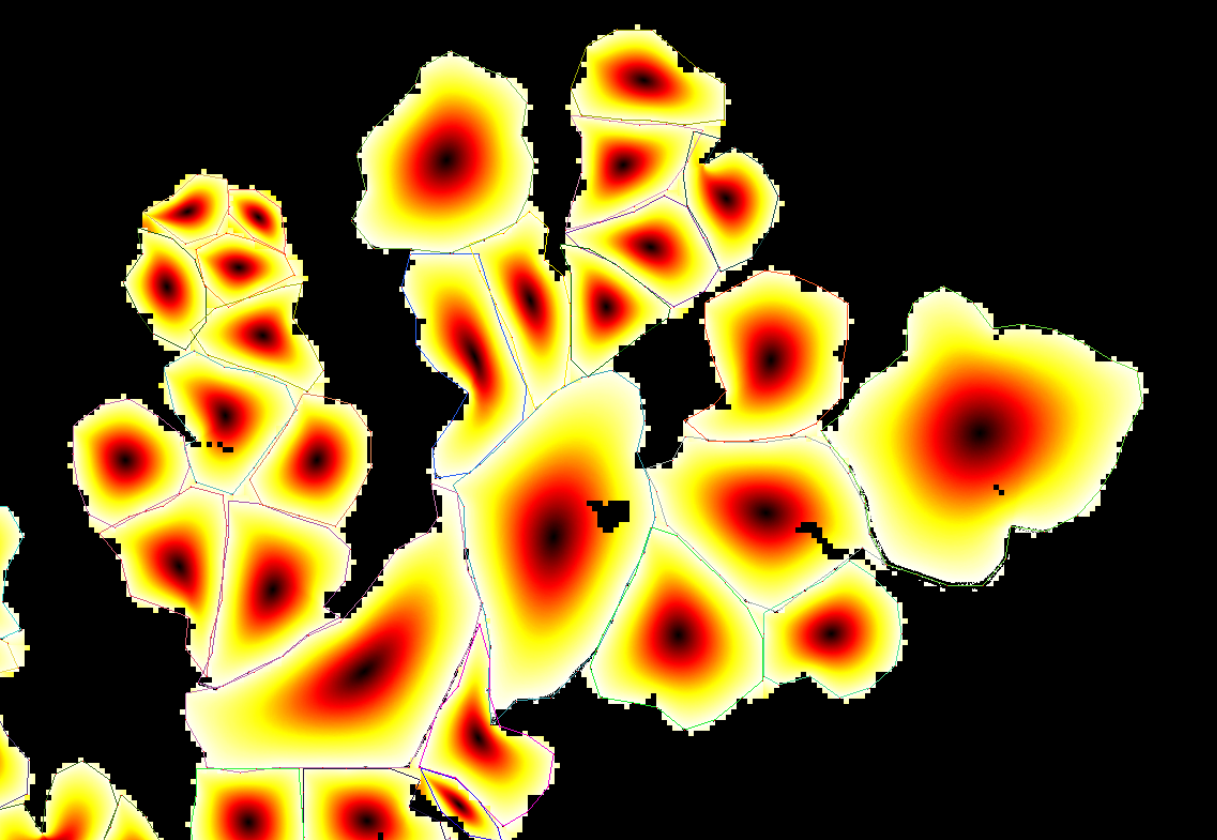
\includegraphics[width=0.6\linewidth]{img/param/concave_hull/clusters_concave_hull.png}
    \caption{Exemple d'un conjunt de clústers texturats usant l'envolupant còncau com a \textit{hull}. Font: elaboració pròpia.}
    \label{fig:concave-hull-clusters}
\end{figure}

El que ens permet el \textit{concave hull} és resseguir de manera més fidel la forma original del clúster que volem texturar, com és el cas de la figura \ref{fig:concave-hull}. Això fa que la textura es deformi molt més que en alguns casos pot quedar exagerat, però no talla la imatge com en el cas de l'envolupant convexa.

\begin{figure}[H]
    \centering
    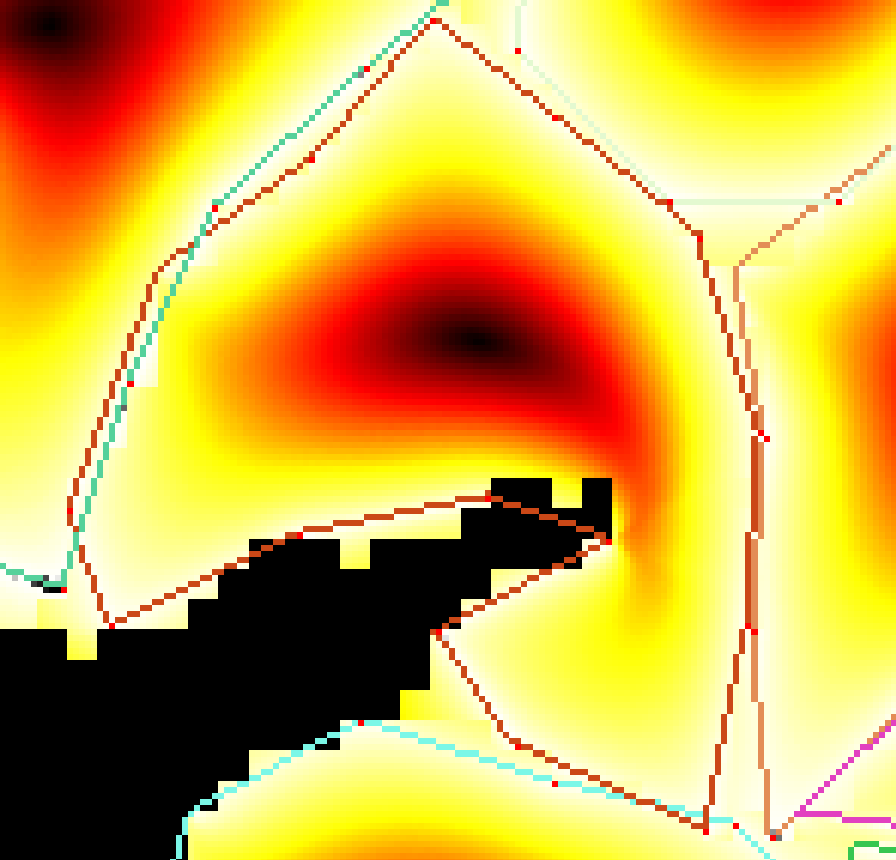
\includegraphics[width=0.5\linewidth]{img/param/concave_hull/concave_hull.png}
    \caption{Exemple d'un clúster texturat amb el seu \textit{concave hull}. En aquest cas, per fer el \textit{hull} s'han fet servir 1 de cada 40 punts del contorn complet. Font: elaboració pròpia.}
    \label{fig:concave-hull}
\end{figure}
\newpage

\section{Pipeline}

\subsection{Obtenció de les textures del liquen}

Per tal de poder fer un liquen que tingui una textura realista necessitàvem una textura base per a poder pintar els clústers que formen el liquen. Convenia que fos una textura circular, ja que en el pas de subdividir el liquen s'intenta tenir uns clústers tan circulars com sigui possible, i que fos procedural, és a dir, que en puguem canviar característiques fàcilment, com ara el color, la rugositat...

El millor candidat que vaig trobar que complia aquests dos requisits va ser una texura en format Substance \cite{adobeFolioseLichen}. El format Substance permet generar textures de manera dinàmica utilitzant programes com Blender a través d'un connector (vegeu la imatge \ref{fig:og-texture}). 

El resultat és molt realista quan el comparem la imatge d'un sol liquen real \ref{fig:real-lichen}.

\begin{figure}[H]
     \centering
     \begin{subfigure}[b]{0.3\textwidth}
         \centering
         
\includegraphics[width=\textwidth]{img/param/original_lichen_texture/lichen_color_map.png}
         \caption{Color.}
         \label{fig:y equals x}
     \end{subfigure}
     \hfill
     \begin{subfigure}[b]{0.3\textwidth}
         \centering
         
\includegraphics[width=\textwidth]{img/param/original_lichen_texture/lichen_displacement_map.png}
         \caption{Desplaçament.}
         \label{fig:three sin x}
     \end{subfigure}
     \hfill
     \begin{subfigure}[b]{0.3\textwidth}
         \centering
         
\includegraphics[width=\textwidth]{img/param/original_lichen_texture/lichen_normal_map.png}
         \caption{Normals.}
         \label{fig:five over x}
     \end{subfigure}
        \caption{Exemple dels diferents mapes de textura generats a partir de la textura en format Substance. Font: elaboració pròpia.}
        \label{fig:og-texture}
\end{figure}


\subsection{Escalat}

Abans d'aplicar la parametrització es fa un escalat dels clústers que s'obtenen de la subdivisió, perquè si no la resolució a la qual es generen aquests és massa baixa perquè es vegin els detalls de la textura original. A més, fer l'escalat en aquest punt de l'execució fa que no augmenti el temps que tardarien a executar-se la generació del liquen i la subdivisió. L'escalat que es fa és molt senzill i consisteix a multiplicar cada píxel per una ràtio determinada en amplada i alçada.

\subsection{Parametrització amb textura intermediària \label{sec:param-proxy}}

Tal com he explicat a la secció del MVC, per tal de poder aplicar la funció de traducció que ens dona necessitem tenir el mateix nombre de vèrtexs en el polígon contenidor de la textura original i del clúster. En el cas que es faci servir el \textit{convex hull} per calcular el polígon contenidor d'un dels dos polígons es necessita una textura intermediària, ja que l'algorisme de Graham Scan retorna el nombre mínim de vèrtexs que defineixen el polígon, que pot diferir entre els dos polígons, en aquest cas la textura original i els clústers.

La textura intermediària o \textit{proxy} que he escollit té la forma d'un cercle, ja que és una forma similar a la textura original \ref{fig:og-texture} i a més ens permet definir arbitràriament el nombre de vèrtexs del seu \textit{hull} i la proporció de les arestes d'aquests. És a dir, si volem $n$ vèrtexs simplement he dividit $\alpha_i = 2 \pi / n \cdot i$ per saber quin angle difereix entre cada vèrtex i després calcular el punt:
$$vx_i = \cos(\alpha_i) \cdot r + cx$$
$$vy_i = \sin(\alpha_i) \cdot r + cy$$
on $cx$ i $cy$ són les coordenades del centre del cercle i $r$ el radi d'aquest.
I si es vol que segueixi unes proporcions donades perquè hi hagi menys deformacions $\alpha_i = {\sum_{i=1}^{n} p_i} \cdot 2\pi $,
on $p$ és una llista amb les proporcions que ha de tenir cada un de les arestes del \textit{hull}.

Un cop sabem com calcular el \textit{hull} del cercle intermedi ja podem fer la traducció completa textura $\rightarrow$ clúster:

\begin{itemize}
    \item Calculem el \textit{hull} de la textura original i ens retorna un polígon amb $n$ costats. Calculem el \textit{hull} del cercle \textit{proxy} a partir dels $n$ costats que defineixen l'envolupant de la textura original.
    \item Utilitzant el MVC per cada punt del cercle calculem el punt que li correspon de la textura original, n'obtenim el color, la normal i el desplaçament i l'apliquem al punt del cercle.
    \item Calculem el \textit{hull} del clúster que volem texturar i en retorna una llista de $m$ vèrtexs. Tornem a calcular el \textit{hull} del cercle però ara a partir dels $m$ costats del \textit{hull} del clúster.
    \item Utilitzant el MVC per cada punt del clúster calculem el punt objectiu del circle, n'obtenim el color, la normal i el desplaçament i l'apliquem al punt del clúster.
\end{itemize}


\subsection{Anàlisi dels resultats parcials}

Per tal de poder comprovar quin és el mètode d'obtenció del polígon contenidor que dona millors resultats, he fet el test amb totes les combinacions possibles per calcular el \textit{hull} mostrant el mateix clúster. En aquest cas només mostrem els resultats pel que fa al mapa de color, però en fer la traducció també generem els mapes de normals, desplaçament i opacitat que ens serveixen per a la visualització en models 3D i il·luminació. Generar aquests mapes no suposa cap pas extra perquè les coordenades d'aquests mapes coincideixen amb els del mapa de color.

\subsubsection{Líquen convex hull - Clústers convex hull}

Les deformacions d'aquest mètode són prou correctes, el problema principal amb aquest mètode és que la textura pot quedar tallada depenent de la forma del \textit{hull}. A més quan la textura queda tallada es veuen quadrats que són la forma original del clúster (vegeu la imatge \ref{fig:liquen-cxh-cxh}).

\begin{figure}[H]
     \centering
     \begin{subfigure}[b]{0.3\textwidth}
         \centering
        
\includegraphics[width=\textwidth]{img/param/lichen_edges_cluster_edges/circle_proxy_color_map.png}
        \caption{Cercle \textit{proxy}.}
         \label{fig:proxy-cxh}
     \end{subfigure}
     \hspace{1cm}
     \begin{subfigure}[b]{0.3\textwidth}
         \centering
        
\includegraphics[width=\textwidth]{img/param/lichen_hull_cluster_hull/close_up.png}
        \caption{Liquen texturat.}
         \label{fig:liquen-cxh-cxh}
     \end{subfigure}
    \caption{Exemple d'un clúster texturat utilitzant el \textit{convex hull} per la textura i els clústers.}
    \label{fig:three graphs}
\end{figure}

\subsubsection{Líquen convex hull - Clústers concave hull}

Aquest mètode elimina els quadrats que he comentat en el test anterior, ja que s'usa el contorn del clúster i, per tant, la textura no queda tallada. Tot i que la textura queda bastant més deformada, els resultats són creïbles, tal com es veu a la imatge \ref{fig:liquen-cxh-cvh}.

El problema principal amb aquest mètode és que accentua els espais buits entre clústers, això passa per com és el cercle \textit{proxy} (vegeu la imatge \ref{fig:proxy-cxh}), que conté espais buits al voltant del perímetre a causa del \textit{convex hull} de la textura original.  Això es podria solucionar utilitzant una tècnica anomenada \textit{blending} a les fronteres entre clústers. El \textit{blending} consisteix a calcular un color mitjà basant-se en els colors de la frontera. El cercle \textit{proxy} és el mateix que en el test anterior perquè s'utilitza el \textit{convex hull} pel liquen.

\begin{figure}[H]
    \centering
    
\includegraphics[width=0.3\linewidth]{img/param/lichen_hull_clusters_edges/close_up.png}
    \caption{Exemple d'un clúster texturat utilitzant el \textit{convex hull} per la textura i amb el contorn als clústers.}
    \label{fig:liquen-cxh-cvh}
\end{figure}

\subsubsection{Liquen concave hull - Clústers convex hull}

En aquest test passem a utilitzar el contorn per al \textit{hull} de la textura del liquen.  Aquest cas no dona bons resultats en el clúster texturat (vegeu la imatge a \ref{fig:liquen-cvh-cxh}) a causa de la deformació de la textura en passar-la al cercle (vegeu la imatge \ref{fig:proxy-cvh}). Això passa perquè hi ha promunicions que tenen massa pes perquè tenen molt de recorregut en el contorn, tal com es veu a la imatge del cercle intermedi.

\begin{figure}[H]
     \centering
     \begin{subfigure}[b]{0.3\textwidth}
         \centering
         
\includegraphics[width=\textwidth]{img/param/lichen_edges_cluster_hull/circle_proxy_color_map.png}
         \caption{Cercle \textit{proxy}.}
         \label{fig:proxy-cvh}
     \end{subfigure}
     \hspace{1cm}
     \begin{subfigure}[b]{0.3\textwidth}
         \centering
        
\includegraphics[width=\textwidth]{img/param/lichen_edges_cluster_hull/close_up.png}
        \caption{Liquen texturat.}
         \label{fig:liquen-cvh-cxh}
     \end{subfigure}
    \caption{Exemple d'un clúster texturat utilitzant el contorn per la textura i el contorn per als clústers. Font: elaboració pròpia.}
    \label{fig:three graphs}
\end{figure}

\subsubsection{Líquen concave hull - Clústers concave hull}

Aquest test té els mateixos problemes que l'anterior i els quadrats de la superfície apareixen ni que s'utilitzi el contorn per al \textit{hull} del clúster (vegeu la imatge \ref{fig:liquen-cvh-cvh}). Això passa per com és la textura intermèdia (vegeu la imatge \ref{fig:proxy-cvh}) perquè la textura intermèdia té unes regions del perímetre que estan pintades completament, cosa que fa que es pintin de color tots els punts del clúster.

\begin{figure}[H]
    \centering
    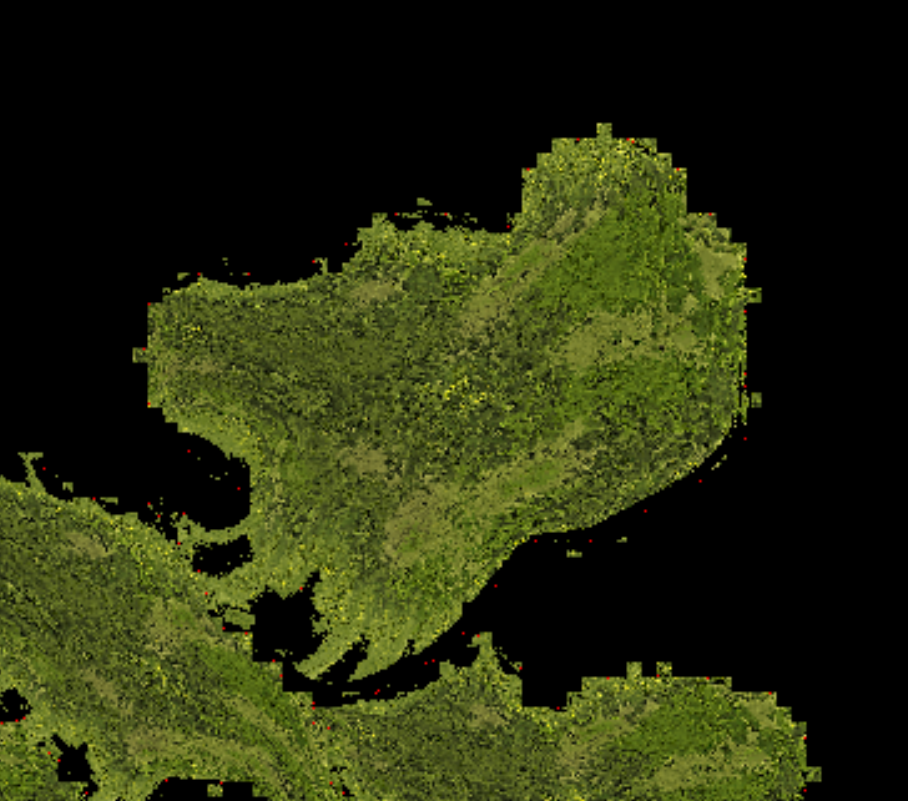
\includegraphics[width=0.3\linewidth]{img/param/lichen_edges_cluster_edges/close_up.png}
    \caption{Exemple d'un clúster texturat utilitzant el contorn per la textura i pels clústers.}
    \label{fig:liquen-cvh-cvh}
\end{figure}

\subsubsection{Conclusions dels resultats parcials}

Els tests de les diferents combinacions ens dona les eines necessàries per triar quina és la millor versió o la que millor s'adapta a les meves necessitats. El cas que genera una textura més realista és la combinació d'usar el \textit{convex hull} per al liquen i el \textit{conacve hull} per als clústers sobretot perquè no genera els quadrats que es veuen en els nostres casos. El problema que té és que si no s'aplica el \textit{blending} els clústers estan inconnexos. És per això que per la visualització final he decidit usar la combinació de \textit{convex hull} en el liquen i els clústers perquè no crea moltes deformacions i els clústers tenen més connectivitat entre ells. Els casos en què s'usa la \textit{concave hull} per al liquen queden descartats perquè els resultats estan massa deformats.

\newpage

\section{Resultats}

Després d'haver vist els passos fer generar un liquen realista, a continuació, mostrem l'evolució d'un sol liquen des del creixement fins a la visualització d'aquest en un model d'herència cultural.

Primer de tot tenim la generació del creixement del liquen utilitzant la meva versió del DLA, en aquest cas el liquen té una mida final de 2000 punts (vegeu figura \ref{fig:dla-growth}).

\begin{figure}[H]
     \centering
     \begin{subfigure}[b]{0.3\textwidth}
         \centering
         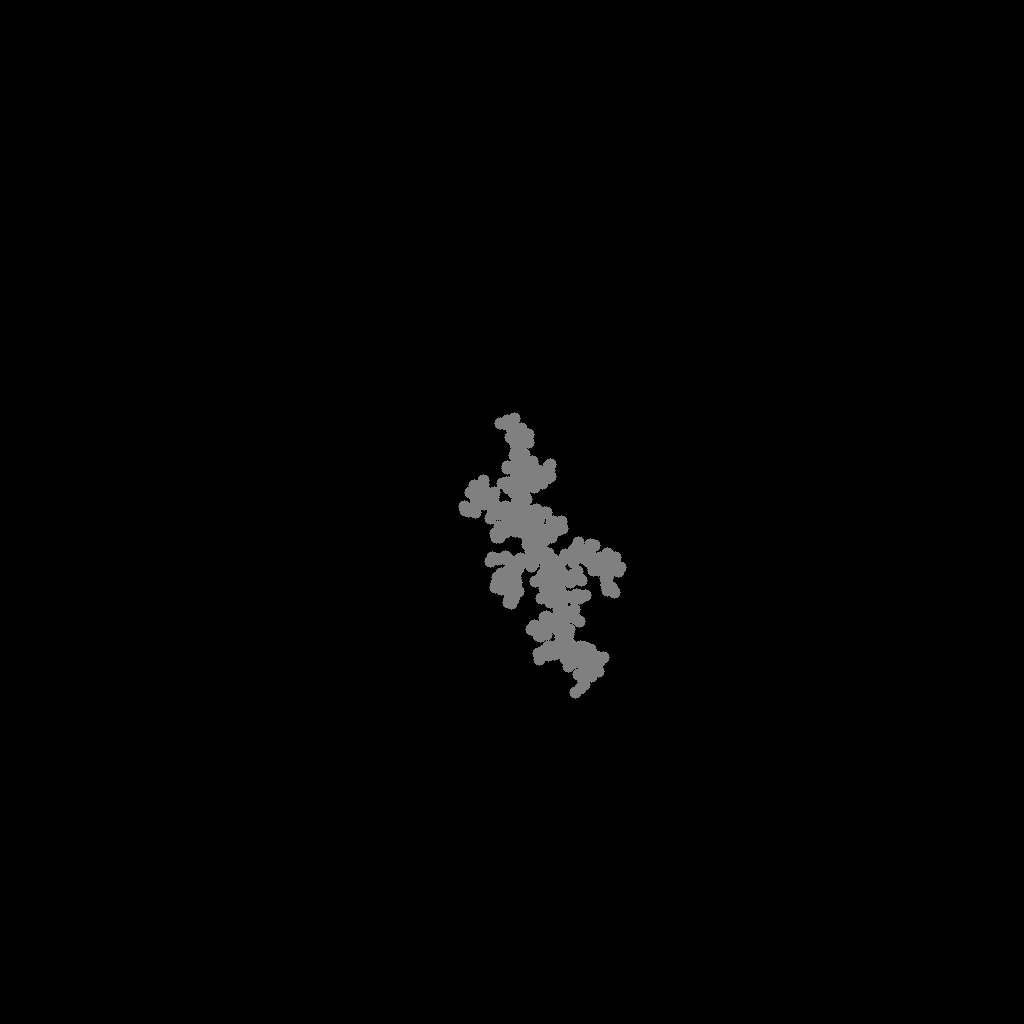
\includegraphics[width=\textwidth]{img/final_results/dla_500_color_map.png}
         \caption{500 punts.}
         \label{fig:y equals x}
     \end{subfigure}
     \hfill
     \begin{subfigure}[b]{0.3\textwidth}
         \centering
         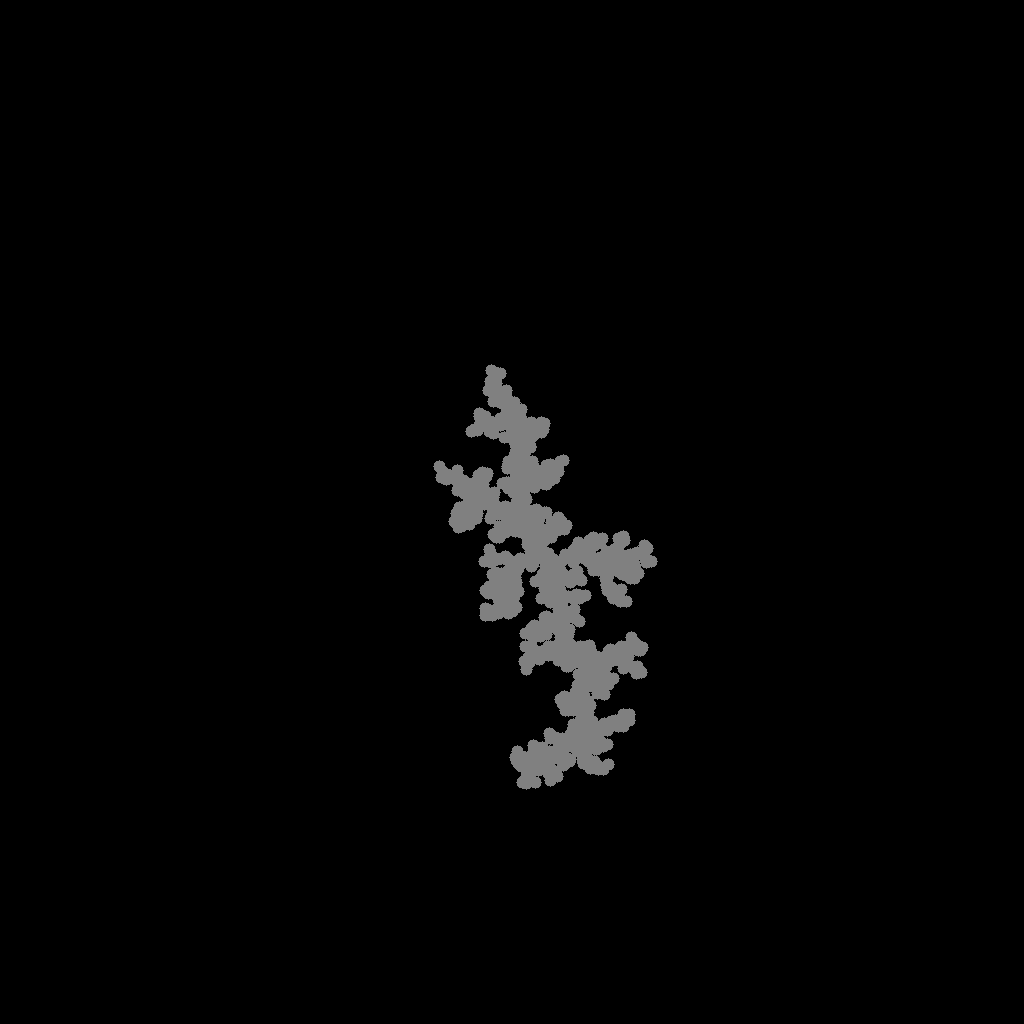
\includegraphics[width=\textwidth]{img/final_results/dla_1000_color_map.png}
         \caption{1000 punts.}
         \label{fig:three sin x}
     \end{subfigure}
     \hfill
     \begin{subfigure}[b]{0.3\textwidth}
         \centering
         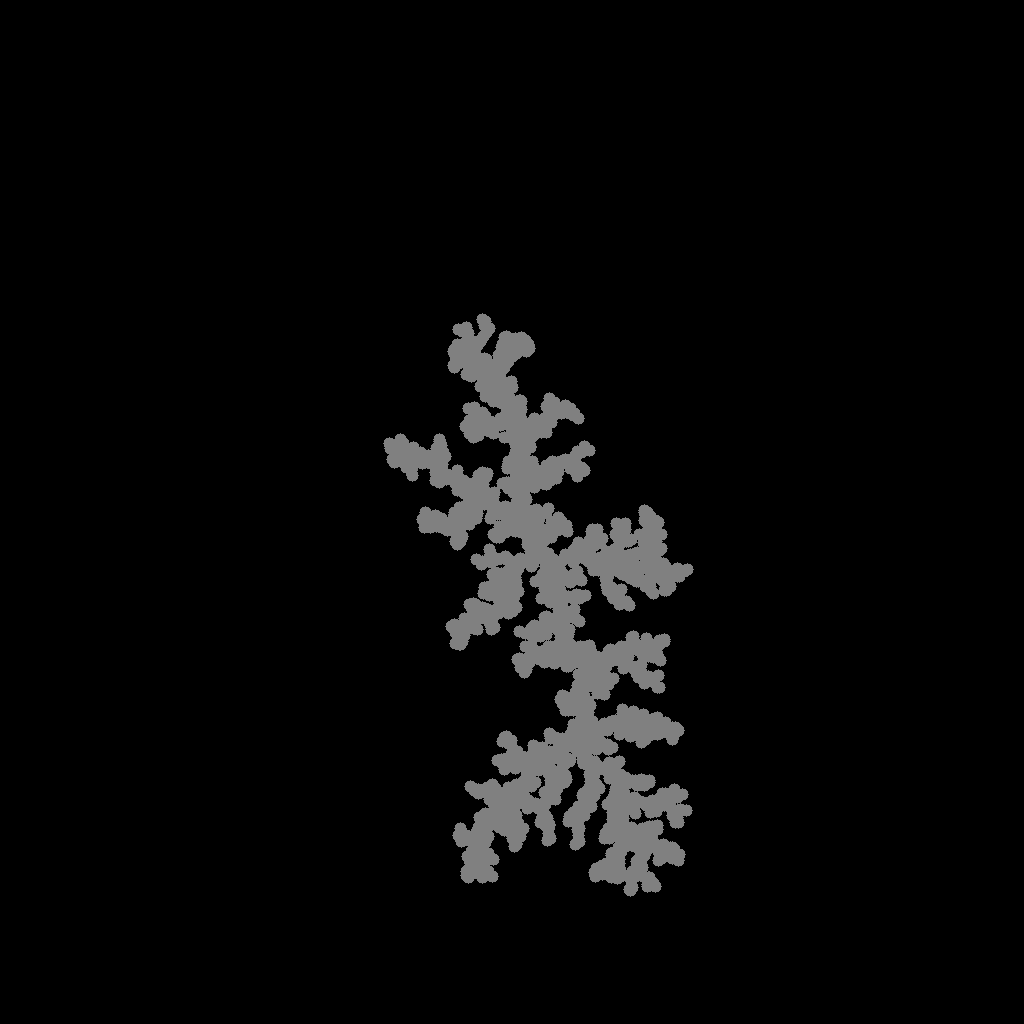
\includegraphics[width=\textwidth]{img/final_results/dla_2000_color_map.png}
         \caption{2000 punts.}
         \label{fig:five over x}
     \end{subfigure}
        \caption{Exemple de l'evolució del creixement del liquen. Font: elaboració pròpia.}
        \label{fig:dla-growth}
\end{figure}

Un cop he obtingut el liquen final, el subdividim usant l'algorisme KMeans. Primer fent una subdivisió en 40 clústers, i després subdividir els clústers que tenen una circularitat inferior a 0.8 que ens acaba donant el resultat de la dreta de la figura \ref{fig:resultats-kmeans}.

\begin{figure}[H]
     \centering
     \begin{subfigure}[b]{0.4\textwidth}
         \centering
         
\includegraphics[width=\textwidth]{img/final_results/first_color_map.png}
         \caption{Primera subdivisó del liquen.}
         \label{fig:y equals x}
     \end{subfigure}
     \hfill
     \begin{subfigure}[b]{0.4\textwidth}
         \centering
         
\includegraphics[width=\textwidth]{img/final_results/final_color_map.png}
         \caption{Subdivisó final del liquen.}
         \label{fig:three sin x}
     \end{subfigure}
        \caption{Exemple de l'evolució del creixement del liquen. Font: elaboració pròpia.}
    \label{fig:resultats-kmeans}
\end{figure}

Un cop he subdividit el liquen toca texturar-lo, en aquest cas la textura original és un liquen de color verd i com a parametrització he utilitzat la \textit{convex hull} en la textura original i en els clústers (vegeu la imatge \ref{fig:texturat-final}).

\begin{figure}[H]
    \centering
    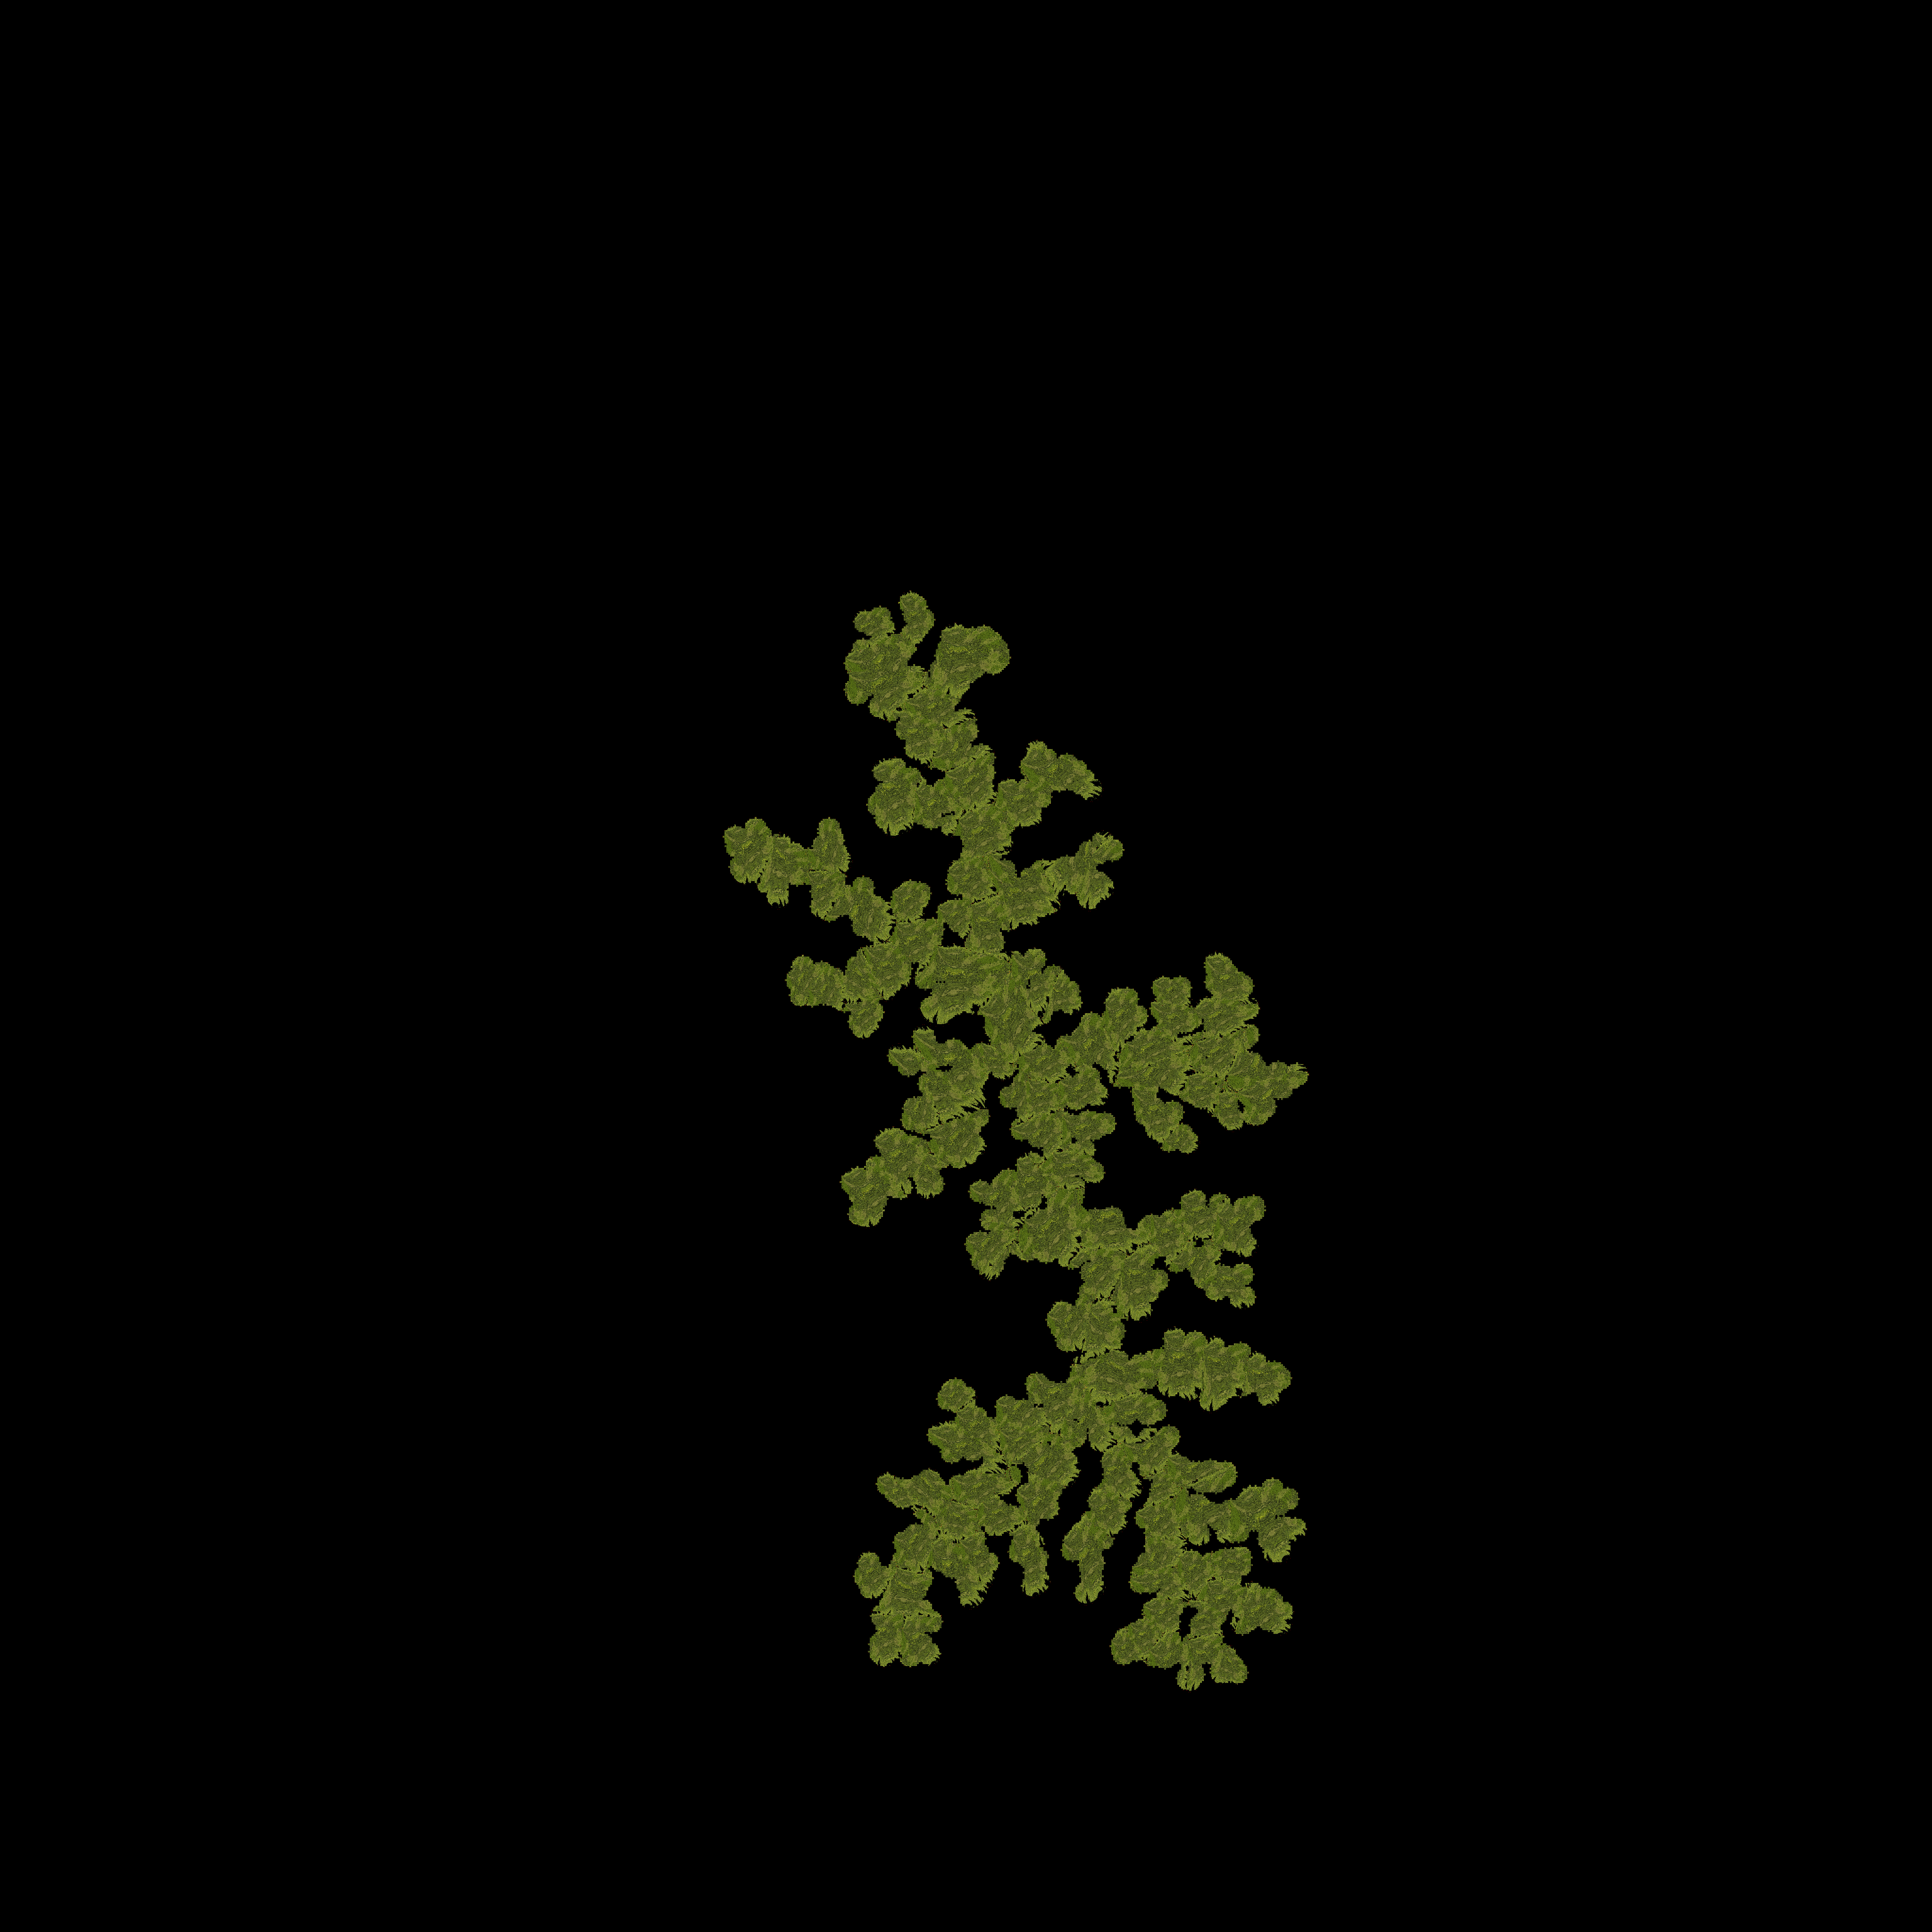
\includegraphics[width=0.4\linewidth]{img/final_results/textured_color_map.png}
    \caption{Liquen texturat. Font: elaboració pròpia.}
    \label{fig:texturat-final}
\end{figure}

Finalment, he afegit dos líquens a dues parets diferents del model virtual de Pedret, desenvolupat per l'EHEM \cite{EHEM}, mitjançant Blender. Aquest procés és molt senzill, ja que quan he acabat de generar els líquens tenim tots els mapes de textura que necessitem per visualitzar-lo sobre el model de Pedret: el mapa de normals per una il·luminació realista del liquen, el mapa de desplaçament per simular la tridimensionalitat del liquen i finalment el mapa d'opacitat per eliminar les parts dels altres mapes que no formen part del liquen. Per configurar la texturació d'un pla en el meu cas, a Blender es configura amb un mapa com el de la figura \ref{fig:shaders-blender}.

\begin{figure}[H]
    \centering
    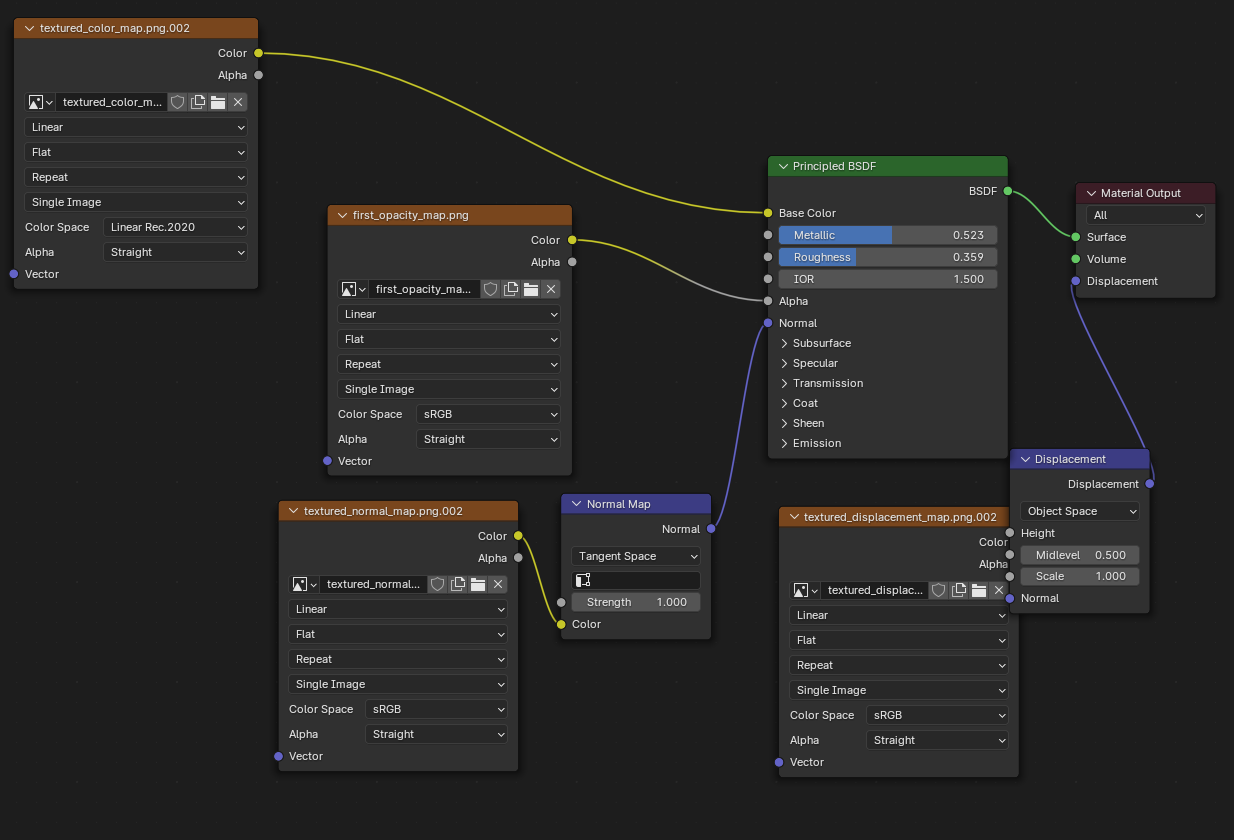
\includegraphics[width=0.7\linewidth]{img/misc/blender.png}
    \caption{Mapa de configuració de textures d'un pla a Blender per obtenir un liquen. Els rectangles de color taronja són les imatges dels diferents mapes de textura que estan connectats amb el \textit{field} corresponent. En el cas de l'opacitat està connectat amb l'alpha perquè és el valor que indica la transparència.}
    \label{fig:shaders-blender}
\end{figure}

Els resultats dels líquens queden realistes perquè s'integren correctament a les parets del model i s'adapten a les condicions de llum on se situa aquest gràcies al mapa de normals (vegeu les imatges \ref{fig:pedret-1} i \ref{fig:pedret-2}). A més, el mapa de desplaçament dona tridimensionalitat el liquen, cosa que fa que el liquen no sembli simplement una pintura sobre la paret. I si es vol canviar l'aparença dels líquens un cop estan sobre el model de Pedret, al mapa de configuració de textures del Blender es poden modificar la rugositat i la metal·licitat.

Les textures dels líquens s'adapten correctament a les parets perquè la superfície es plana. Però podria donar-se el cas que les parets tenen deformacions (per augmentar-ne el realisme) i seria interessant que la \textit{pipeline} generes una textura que s'adapta a la superfície on es troba el liquen.

\begin{figure}[H]
    \centering
    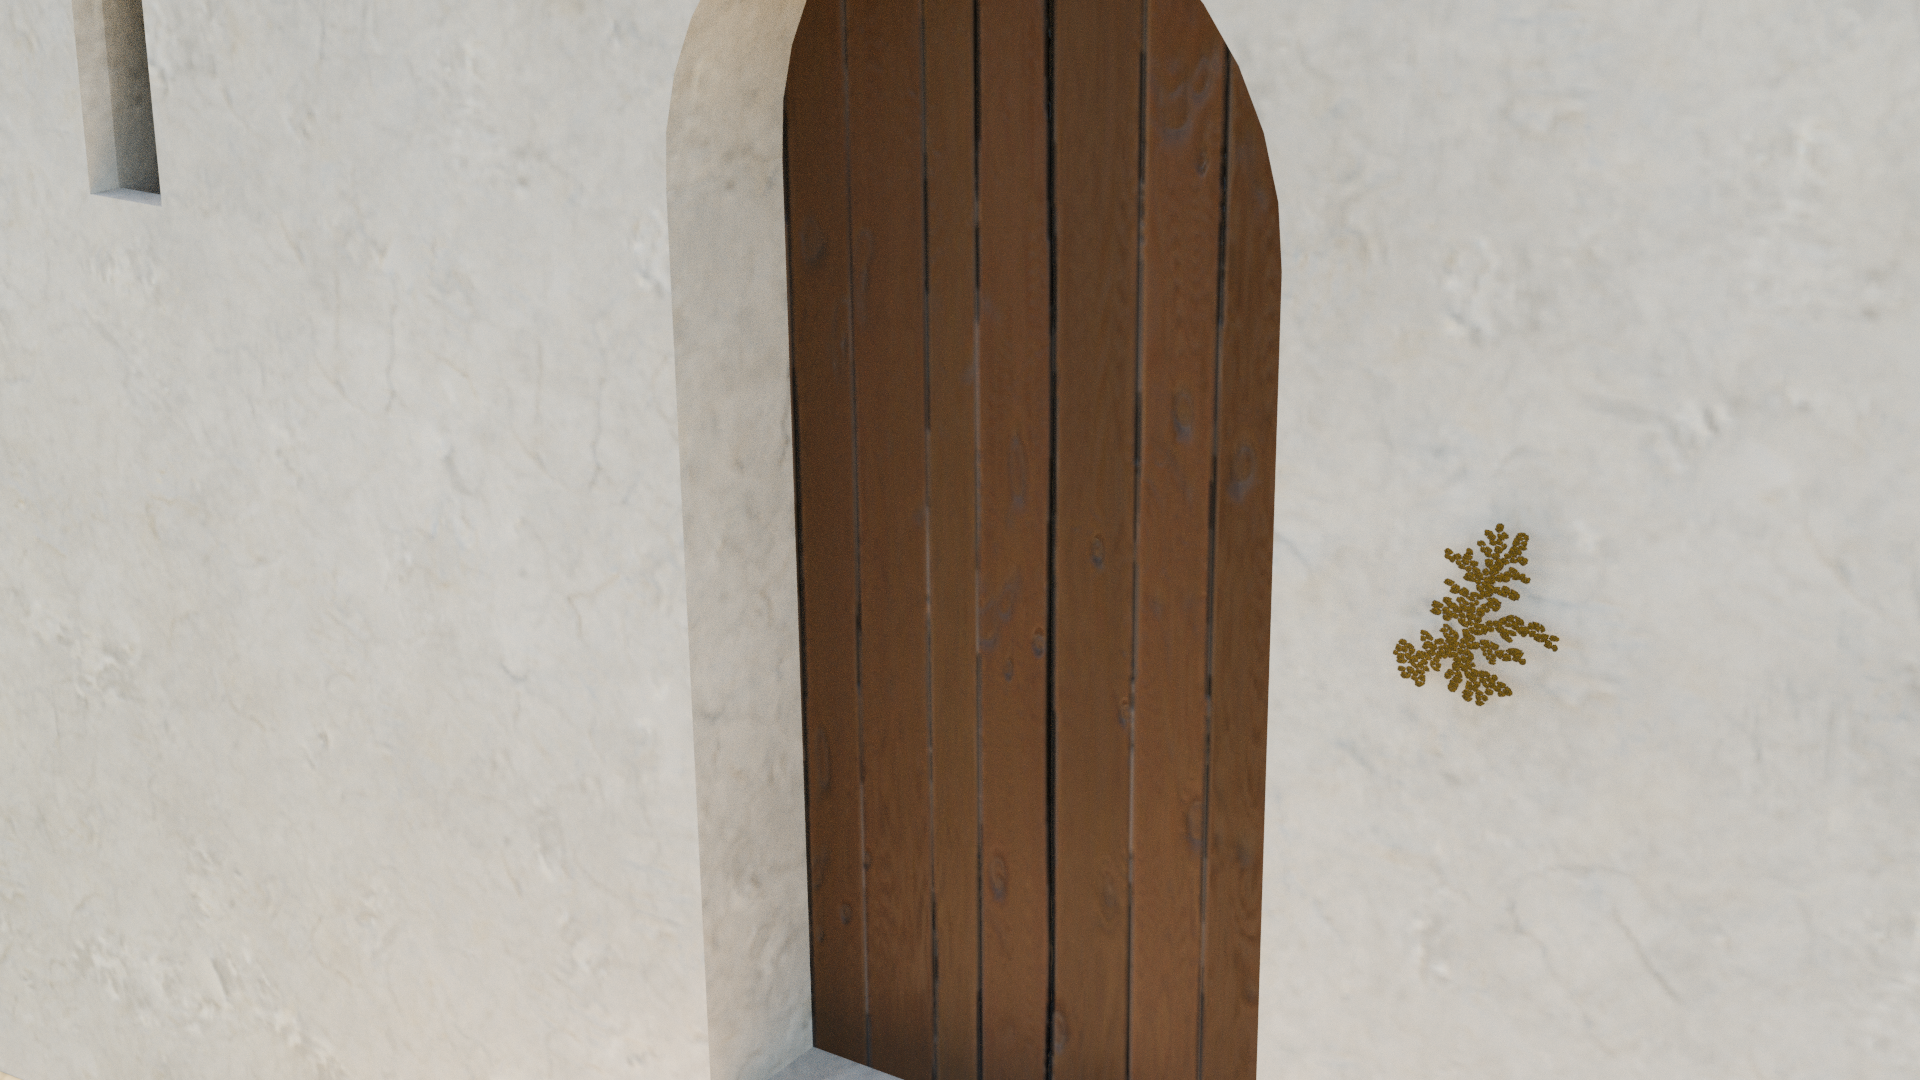
\includegraphics[width=0.8\linewidth]{img/final_results/pedret.png}
    \caption{Exemple d'un liquen en una de les parets del model de Pedret renderitzat mitjançant Blender. Font: elaboració pròpia.}
    \label{fig:pedret-1}
\end{figure}

\begin{figure}[H]
    \centering
    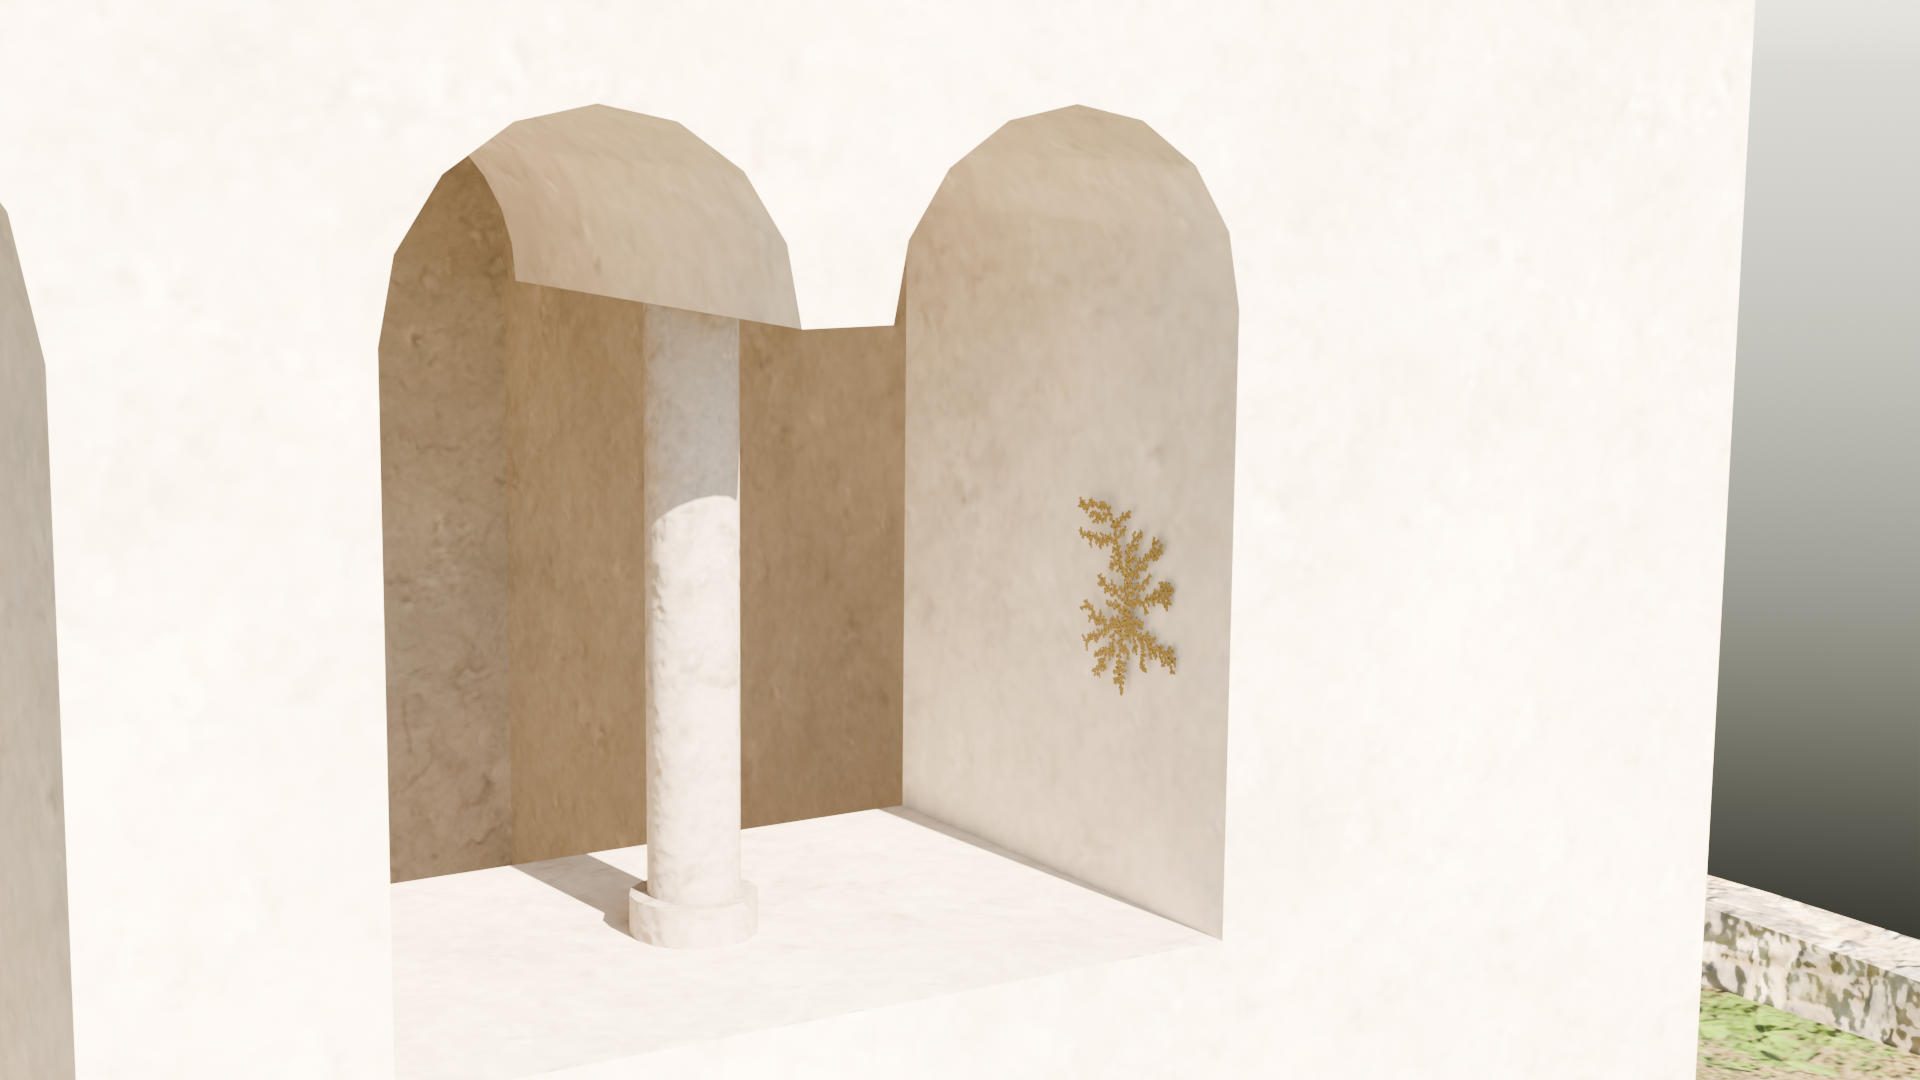
\includegraphics[width=0.8\linewidth]{img/final_results/pedret_1.png}
    \caption{Exemple d'un liquen en una de les parets del model de Pedret renderitzat mitjançant Blender. Font: elaboració pròpia.}
    \label{fig:pedret-2}
\end{figure}

\newpage

\section{Conclusions}

Els objectius principals d'aquest treball eren generar formes realistes de líquens i a partir d'aquestes formes crear models realistes que després es puguin usar en els models d'herència cultural.

Pel que fa al primer objectiu, he aconseguit implementar l'algorisme DLA amb paràmetres per a controlar el creixement dels líquens, fer les modificacions pertinents per millorar els resultats i finalment fer tests per tal de poder validar aquests paràmetres.

En el cas del segon objectiu, finalment ha sigut en el que he hagut de dedicar més temps, ja que ni que la \textit{pipeline} només té dos passos principals que són la subdivisió del liquen i la parametrització, són prou complexos.  Per la subdivisió del liquen he fet diferents proves per tal de veure quina era la millor implementació de l'algorisme KMeans que s'adaptés a les nostres necessitats i finalment he proposat un algorisme que genera clústers majoritàriament circulars. Pel que fa a la parametrització de textures, he implementat i fet tests a diferents tècniques per traduir coordenades de textures a polígons. Aquesta traducció l'he fet mitjançant el MVC i modificant la manera en què es parametritza la forma de la textura i la forma dels clústers, per al que he implementat l'algorisme de Graham Scan i el que he anomenat \textit{concave hull}, en contraposició al \textit{convex hull}.

Els resultats del treball han estat satisfactoris perquè compleixen l'objectiu principal que és simular el creixement de líquens i generar visualitzacions realistes d'aquests. El DLA genera bons resultats els quals l'usuari pot modificar gràcies a la parametrització i la \textit{pipeline} de texturació crea les textures necessàries per a la visualització realista de manera molt senzilla per a l'usuari. 

\subsection{Treball futur}

Tot i que els resultats són satisfactoris, perquè el temps del treball és limitat, hi ha diverses seccions en què es pot ampliar el treball que he fet. La que considero en la que es pot fer més avenços és en la visualització final dels líquens perquè amb els resultats que he obtingut els clústers sembla que no tinguin continuïtat i que el liquen sigui un conjunt d'illes aïllades. Com que els tests amb les diferents maneres de parametritzar ja estan fets, el que faltaria és triar el mètode que doni més bons resultats i aplicar tècniques, com ara el \textit{blending} per omplir els espais buits que fan que els clústers estiguin separats.

En l'apartat del DLA es podrien fer millores pel que fa al rendiment, ja que com que no vaig obtenir bons resultats amb la generació de partícules proposada per Michael S. Floater \cite{FLOATER200319}, vaig implementar el moviment més senzill que fa que es tardi més a agregar noves partícules. Es podria, o bé, veure que va fallar en la meva implementació o buscar mètodes diferents.

Pel que fa a la secció de subdivisió dels clústers, crec que és la més completa, però també si podrien fer millores. Una de les idees per millorar l'algorisme és afegir un factor de circularitat durant el creixement dels clústers, és a dir, agregar primer als clústers les partícules que fan que el clúster sigui més circular. Aquesta idea de circularitat es podria estendre a formes de qualsevol mena, perquè en el cas de tenir una textura que no sigui circular, l'algorisme actual funcionaria, però les deformacions serien massa exagerades.

\newpage

\bibliography{biblio}

\addcontentsline{toc}{section}{Referències}

\bibliographystyle{plain}

\newpage

\section{Apèndix}

\subsection{Implementació}

Podeu trobar tot el codi utilitzat en aquest treball a GitHub \url{https://github.com/rocsalvador/Tesi}.

\end{document}
